\documentclass[a4paper,12pt]{report}
\usepackage{hyperref}
\usepackage{graphicx}
\graphicspath{ {./} }
\usepackage[utf8]{inputenc}
\usepackage{listings, listings-rust}
\usepackage{color, copyrightbox}

\usepackage[
backend=biber,
style=numeric,
sorting=nyt
]{biblatex}
\addbibresource{bib.bib}

\definecolor{dkgreen}{rgb}{0,0.6,0}
\definecolor{gray}{rgb}{0.5,0.5,0.5}
\definecolor{mauve}{rgb}{0.58,0,0.82}
\lstset{frame=tb,
  language=Java,
  aboveskip=3mm,
  belowskip=3mm,
  showstringspaces=false,
  columns=flexible,
  basicstyle={\small\ttfamily},
  numbers=none,
  numberstyle=\tiny\color{gray},
  keywordstyle=\color{blue},
  commentstyle=\color{dkgreen},
  stringstyle=\color{mauve},
  breaklines=true,
  breakatwhitespace=true,
  tabsize=3
}

\title{
    \begin{figure}[hbt!]
        \centering
        
\includegraphics[width=300pt]{pandit.png}
    \end{figure} 
    A Distributed Service-Level Proxy}
\author{
    \textbf{Eric Gerard Moynihan}
\\\\\small{B.Sc. Computer Science - Final Year Project}
\\\\\small{Prof. Dirk Pesch}
\\\\\small{University College Cork}
}
\date{April 2022}

\begin{document}

\pagenumbering{roman}

\maketitle

\chapter*{Abstract}
Pandit transfers abstract data between applications on different servers. It lives on each server and listens for requests by applications on that server.

There are two types of applications that run on the servers: clients and 'servers'. Clients query data and 'servers' provide said data. Pandit acts as a middle-man for these queries.

\subsection*{Services}

Pandit provides 'services' to clients. A service is an abstraction on top of a 'server' that just focuses on the data provided by the server.

Services are defined in a 'gRPC \cite{grpc} Proto file \cite{protobuf}' file that both the client and Pandit have access to; so both know the structure of a particular service.

Pandit handles the querying and conversion of data from the servers; this allows the clients to receive data in a uniform format.

\subsection*{Caching}

Since Pandit knows how to translate the data; Pandit knows when it gets the same request for data twice. This allows it to store previously seen responses. If it gets the same request twice, it will return the cached data without adding extra load to the server.

\chapter*{Declaration of Originality}
In signing this declaration, you are conforming, in writing, that the submitted work is entirely your own original work, except where clearly attributed otherwise, and that it has not been submitted partly or wholly for any other educational award.
I hereby declare that:
\begin{itemize}
    \item this is all my own work, unless clearly indicated otherwise, with full and proper accreditation;
    \item with respect to my own work: none of it has been submitted at any educational institution contributing in any way to an educational award;
    \item with respect to another’s work: all text, diagrams, code, or ideas,
whether verbatim, paraphrased or otherwise modified or adapted, have
been duly attributed to the source in a scholarly manner, whether
from books, papers, lecture notes or any other student’s work, whether
published or unpublished, electronically or in print.
\end{itemize}

\textbf{Signed:} 
\includegraphics[width=100pt]{sig.png}

\textbf{Date: } 23rd April 2022

\chapter*{Acknowledgements}

Firstly, I would like to thank my supervisor, Professor Dirk Pesch, for helping me every step of the way during this process. 
Every time I had a question regarding the project, Dirk got back to me with a timely response. 
I am also thankful for Dirk taking on this project, as it was proposed by myself. 
Without a supervisor that allowed me to pursue this project, I wouldn't have been able to do it.
For that, I am very thankful.

I would also like to thank Netsoc for providing Netsoc Cloud instances to different deployments of Pandit.
I learned a lot as a member of the Netsoc System Administrator committee for the past few years.
I gained many technical skills in the areas of Code Review, Programming and System Administration.
I also gained teamwork experience during my time there, and for that I am very thankful.

I would also like to thank Google, the company I did my work placement for.
In particular, I would like to thank my host Jose-Luis Izquierdo-Zaragoza for providing me with many hours of learning throughout my work placement.
It was at Google that I learned the power of using code generation and protocol buffers, which is what inspired me to pursue this very project.
For that, I would like to say a big thank you to everyone who helped me during my time there.

\subsection*{External Libraries Used}
I used many external Rust libraries to complete this project. Here is a complete list of them:

\begin{lstlisting}
access-json = "0.1.0"
async-recursion = "1.0.0"
api_proto = { path = "./src/api/proto", package = "api" }
bollard = "0.11"
get_if_addrs = "0.5.3"
clap = { version = "3.1.2", features = ["derive"] }
hostname = "0.3.1"
kube = { version = "0.69.1", features = ["runtime", "derive"] }
k8s-openapi = { version = "0.14.0", features = ["v1_22"] }
log = "0.4.11"
config = "0.11.0"
crossbeam-channel = "0.5.2"
tonic = "0.6.2"
h2 = "0.3"
tower-test = "0.4.0"
num = "0.4"
libc = "0.2"
hyper = { version = "0.14", features = ["full"] }
tokio-postgres = { version = "0.7.5", features = ["with-serde_json-1"] }
postgres-types = "0.2.2"
postgres-protocol = "0.6.3"
sea-query = { version = "^0", features = ["postgres-array"] }
grpcio = { version = "0.10.0", default-features = false, features = ["protobuf-codec"] }
tempfile = "3.3.0"
bytes = "1.1.0"
http = "0.2.6"
tokio = { version = "^1.0.1", features = ["rt", "signal", "time", "io-util", "net", "sync", "tracing"] }
console = "0.15.0"
tokio-test = "0.4.2"
parameterized = "0.3.1"
futures = "0.3"
tracing = "0.1.26"
async-trait = "0.1.52"
serde_json = "1.0"
tracing-subscriber = "0.3.2"
console-subscriber = "0.1.3"
serde-protobuf = "0.8.2"
serde = { version = "1.0.133", features = ["rc"] }
httparse = "1.5.1"
dashmap = { version = "4.0.2", features = ["serde"] }
protobuf = { git = "https://github.com/stepancheg/rust-protobuf.git", tag="v3.0.0-alpha.2", features = ["with-serde"] }
protoc-rust = "2.25.2"
protobuf-parse = { git = "https://github.com/stepancheg/rust-protobuf.git", tag="v3.0.0-alpha.2" }
redis = { version = "0.21.5", features = [ "cluster", "tokio-comp"] }
\end{lstlisting}

\tableofcontents

\listoffigures

\pagenumbering{arabic}

\chapter{Introduction}
Pandit at its core is a \textbf{distributed service-level proxy}.

A \textit{proxy} in this context means an intermediary server that acts as a middle-man between a client requesting some data and the server that is hosting said data.

The proxy will be \textit{service-level} because it will provide an abstraction of the underlying server called a \textit{service} to the clients. This
will be achieved by implementing Pandit in such a way that it is able to parse the data provided by the server and convert it into a uniform machine-readable API.

The proxy will be \textit{distributed} across physical servers. This will allow clients on one physical server to query a Pandit \textit{service}. 
This query will be handled by the Pandit instance on the local machine. 

Pandit will utilise caching \cite{caching} to speed up the query responses, and since it the server with the data could be on any server, Pandit will delegate the request to another physical server's Pandit instance, allowing for the possibility of another cache hit before the request is translated and sent to the server with the data.

\begin{figure}[hbt!]
    \centering
    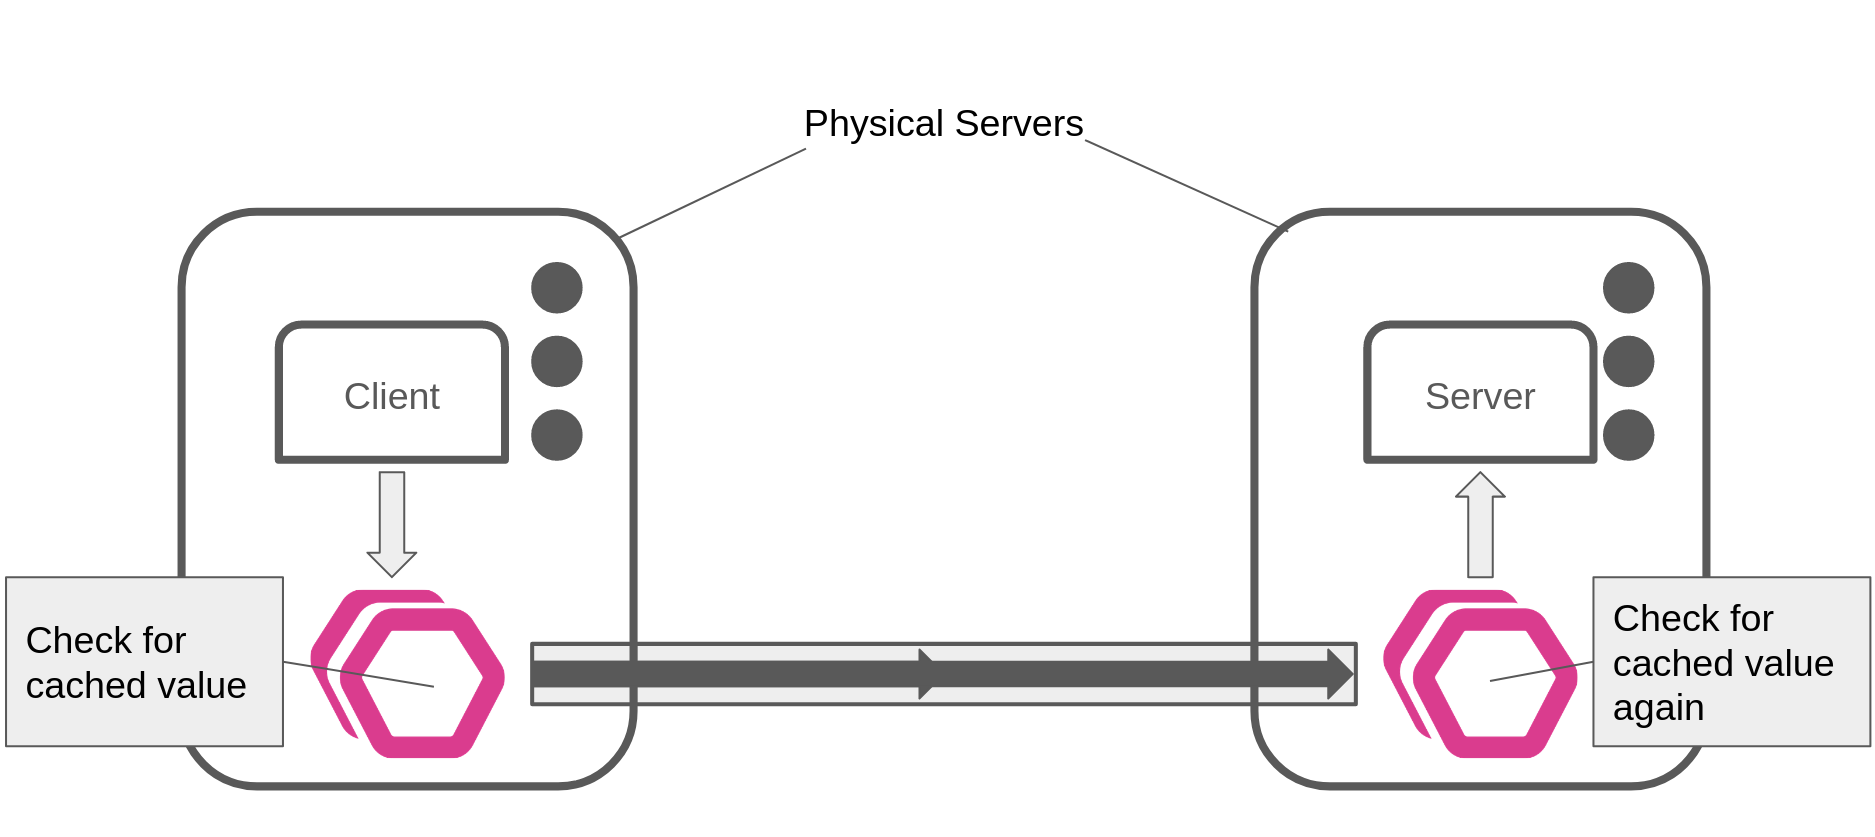
\includegraphics[width=\linewidth]{fig1.png}
    \caption{Basic Distributed Deployment Overview, showing flow of query between two servers.}
    \label{fig:1}
\end{figure}

Since Pandit parses the entire payload, smarter caching strategies can be applied than those provided by traditional proxies.

\chapter{Analysis}

\section{Background}

This project utilises many existing technologies and concepts. Provided below is some background information on these technologies.

\subsection{The Rust Programming Language}

The entire project is implemented using the Rust Programming Language \cite{rust}. Providing fast execution times, compile-time memory safety
and great tooling.

\subsubsection{Type System}
Rust proved to be challenging at times due to its rigid type system. Rust is statically typed; all types must be known on compile-time. Adding to the complexity and development time. Rust reduces the likelihood of runtime errors as a consequence of this. Compared to dynamically typed languages such as Python; Rust provides more efficient, less error-prone code.

\subsubsection{Lifetimes}
Another benefit of Rust would be its \textit{lifetime system \cite{lifetimes}}. Unlike most languages, Rust doesn't have garbage collection. 
Garbage collection is when a program frees up memory by removing objects from the heap. 

Objects in traditional programs are freed from the heap when there is no longer any code that references the object.
A garbage collection routine detects this and frees the memory.
This is computationally expensive because the program has to realise that an object needs to be freed at \textbf{runtime}.

Rust on the other hand does this at \textit{compile-time}. Knowing at what point in the program memory should be freed before it even runs. This removes the need for a garbage collection routine.

It achieves this by introducing the concept of lifetimes. Lifetimes are compiler-enforced rules that ensure that both the programmer and compiler know at what point in the program an object can be freed. 
This is seen from the programmer's perspective as an object going out of scope. 

An object can be \textbf{borrowed} from one lifetime to another. This occurs when a \textbf{reference} to the original value is used in a different scope.
Borrowing an object is allowed when it is \textbf{guaranteed on compile time} that the reference will not outlive the underlying value it's borrowing from.

Take a look at this example:

\begin{lstlisting}[language=Rust]
fn main() {
    let x = "str";
    {
        // new scope
        let y = &x; // borrowing x
        println!("{}", y);
    }
    println!("{}", x);
}
\end{lstlisting}

The value x is borrowed by y, which is in a separate scope and hence, a separate lifetime.
\textit{y} will only live as long as its scope, it will go out of scope before x in this case.
Here we can guarantee that x has a longer lifetime than y, and hence the borrow is allowed.


\subsection{Protocol Buffers}
\label{sec:protobufs}
Protocol Buffers \cite{protobuf} is an open standard for the serialising of structured data.
It is a binary standard, meaning that it defines the serialising of data into a string of binary.

The structure of the data is defined in what is known as a \textit{Proto} file. This file is used by the applications transferring the data to both serialise and deserialise the data. 

The most basic concept in a \textit{Proto} file is a \textit{message}. This defines the basic structure of the serialised data. Here is a basic example of a message:

\begin{lstlisting}
message ExampleRequest {
  int32 id = 1;
  string field1 = 2;
  string field2 = 3;
}
\end{lstlisting}

The reason why each field has a number is that it defines the numeric \textit{tag} that the field will be defined when serialised.
This allows for extremely efficient deserialising; the deserialiser looks up the tag in its local copy of the Proto message in order
to understand how to parse this field. 

Deserialisation is achieved in a single sweep across the binary string.

Text-based formats such as JSON \cite{json} require to be stored in less space-efficient text-based strings; requiring a more complex stack-based approach to parsing. 
Protocol Buffers are far more efficient in comparison because:

\begin{itemize}
    \item The field names are known ahead of time by both the sender and the receiver.
    \item Binary formats are far more space-efficient than text-based formats due to extra bytes being required. Text-based formats struggle to hold non-text based primitive data types such as booleans, floats and integers.
    \item Extra bytes are required to delimit objects in JSON, such as curly braces. The JSON parser does not know the data structure being transferred ahead of time, requiring extra bytes to delimit said data structures.
\end{itemize}

\subsection{gRPC}
\label{sec:grpc}

A Remote Procedure Call (henceforth \textbf{RPC}) is a protocol that allows a program on one computer to call a function and request data from a program on another computer.
gRPC is a protocol made by Google that achieves this by utilising HTTP/2 \cite{http2} and \textit{\nameref{sec:protobufs}}.

It utilises HTTP/2 to allow for the multiplexing of multiple queries into a single TCP connection \cite{tcp}.

\begin{figure}[hbt!]
    \centering
    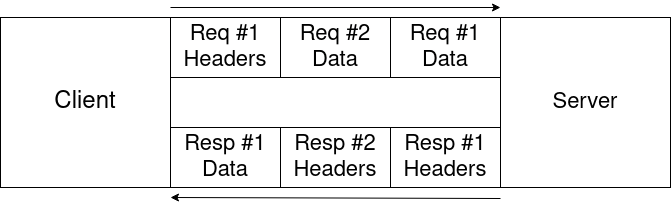
\includegraphics[width=\linewidth]{http2.png}
    \caption{HTTP/2 Multiplexing over a single TCP connection}
    \label{fig:2}
\end{figure}

gRPC extends the \textit{\nameref{sec:protobufs}} format by providing a \textit{Service}. This service defines RPC methods. 
Each method takes a single \textit{message} as its parameters and returns a single \textit{message}.

An example of how a gRPC service can be defined in a Proto file would be the following:

\begin{lstlisting}
service ExampleService {
  rpc GetExample(ExampleRequest) returns (ExampleResponse) {
  }
  rpc GetExample2(ExampleRequest2) returns (ExampleResponse2) {
  }
}
\end{lstlisting}

Therefore, gRPC provides an RPC framework that allows for the efficient transfer of data via the use of Protocol Buffers.

\subsection{Protobuf Options}
\label{sec:options}
\textit{Options} provide a way to embed data inside a Proto specification. They are usually defined inside a package like so:
\begin{lstlisting}
syntax = "proto3";
import "google/protobuf/descriptor.proto";

package pandit;

enum Handler {
  JSON = 0;
  POSTGRES = 1;
};

extend google.protobuf.MethodOptions { 
  Handler handler = 50051; 
}

extend google.protobuf.ServiceOptions { 
  Handler default_handler = 50051; 
}
\end{lstlisting}

This example defines an option called \textit{pandit.handler} that can be added to any gRPC method, and an option called \textit{pandit.default$\_$handler} 
that can be added to any gRPC service. The reason why they are prefixed with \textit{pandit.} is because they are defined inside the package \textit{pandit}.

These options can then be used to add metadata to methods and services, like so:

\begin{lstlisting}
service ExampleService {
  option (pandit.default_handler) = JSON;

  rpc GetExample(ExampleRequest) returns (ExampleResponse) {
    option (pandit.handler) = JSON;
  }
  
}
\end{lstlisting}

Fields and messages can also utilise options like so:

\begin{lstlisting}
// pandit.proto
extend google.protobuf.FieldOptions {
  bool key = 50037; // large number.
}

extend google.protobuf.MessageOptions { 
  string path = 50030; 
}

// message.proto
message ExampleResponse {
  option (pandit.path) = ".obj";
  int32 id = 1 [ (pandit.key) = true ];
  string user = 2;
}
\end{lstlisting}

The reason why options should be defined with a large number is if another imported package also extends some Proto options. If they use the same
number as the previously imported package, it will cause a conflict when parsing the Proto file.

\section{Objectives}
\label{sec:objectives}

\begin{itemize}
    \item Pandit should be designed to be able to proxy any data source, such as REST APIs or SQL databases.
    
    It should read in user-defined \nameref{sec:protobufs} that are extended to provide information on how to parse, cache, and return data to clients.
    
    \item Pandit should provide \textit{Pandit Services}; a \nameref{sec:grpc} service that contains all the necessary data to convert requests and responses to the format required by the server being proxied.
    
    \item Using \nameref{sec:options}, Pandit should provide a way to define the conversion between the application and the Pandit Service.
    
    \item It should be able to cache data based on user-defined caching strategies in a distributed manner.
    
    \item It should be able to be run on a set of networked servers called a cluster.
    
    \item It should support multiple deployment modes, such as Kubernetes \cite{k8s} and Docker \cite{docker}.
\end{itemize}

\section{Approaches}
\subsection{eBPF Approach}
\label{sec:ebpf}
The initial approach to achieving these objectives was to run a daemon on each server. The daemon would load code into a kernel feature called "eBPF" \cite{ebpf}.

eBPF is a technology that allows code to be run inside the Linux kernel. It allows for direct access to features such as network interfaces.

The approach involved using eBPF to hijack packets inside the kernel. Doing some basic parsing inside the kernel, and then sending them to the user-space program.

\begin{figure}[hbt!]
    \centering
    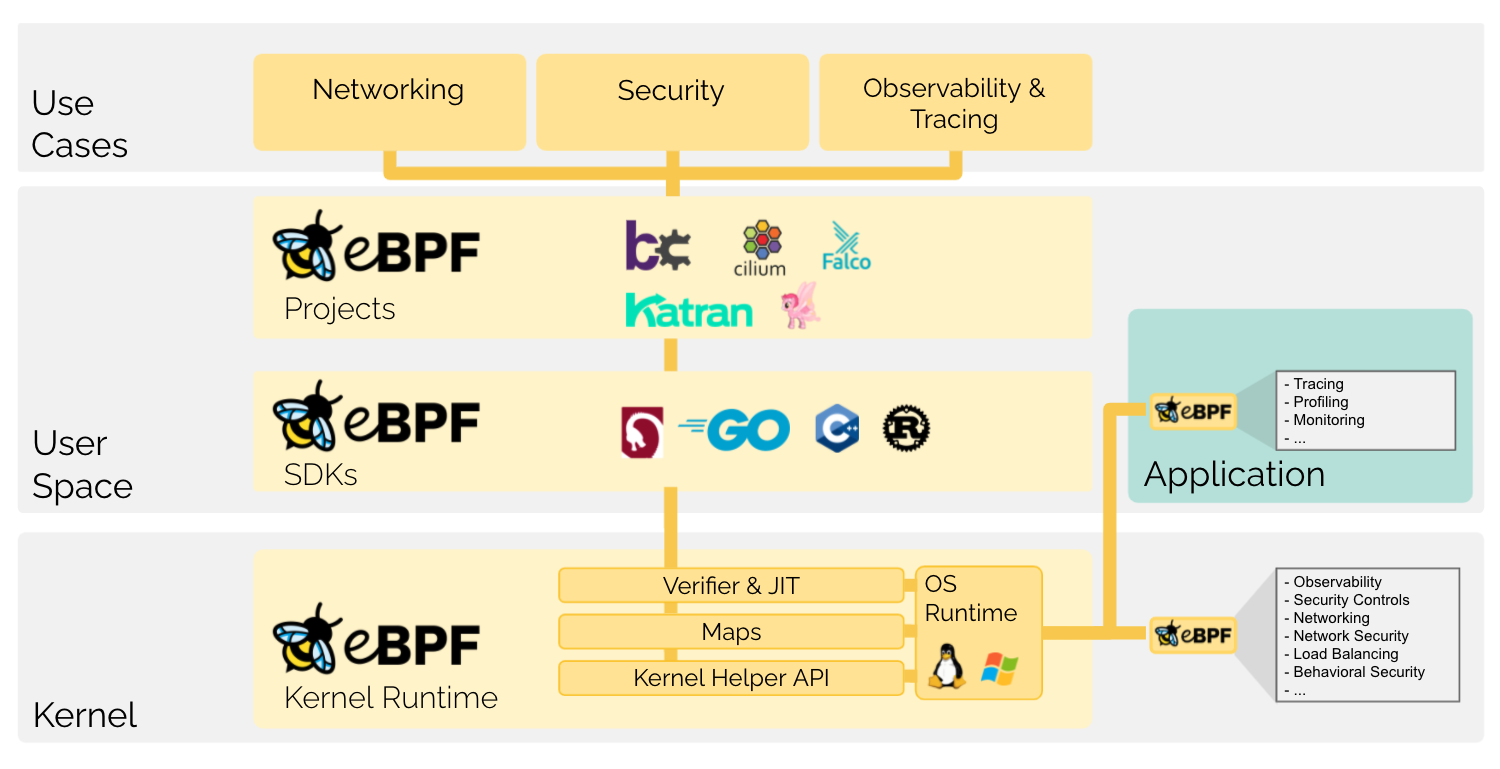
\includegraphics[width=\linewidth]{ebpf.png}
    \caption{Diagram of the eBPF ecosystem. Copyright 2022 eBPF Authors. URL: \href{https://ebpf.io/}{https://ebpf.io/}}
\end{figure}
\newpage

The approach was ultimately scrapped due to the complexities involved with writing an eBPF program. For example:

\begin{itemize}
    \item No shared libraries could be used due to the strict limitations imposed by the eBPF runtime.
    \item The number of instructions a compiled eBPF program could contain was limited to an arbitrary number hardcoded into the kernel. Reducing the ability to perform complex operations.
    \item The number of jumps a program could execute during its lifetime was capped. This limited the processing of payloads in the kernel.
\end{itemize}

\subsection{Userspace gRPC Server approach}
\label{sec:user}
The approach that was decided upon ended up being a lot simpler:
Run a daemon on each server that provides a gRPC server that clients will interface with. 

The daemon will translate the requests to the necessary format. Forwarding them on to the proxied application, caching the results.

\section{Existing Solutions}
\label{sec:solutions}
Service level proxies usually fall into two categories:
\begin{itemize}
    \item A commercial closed-source proxy that focuses on platform-specific use cases.
    \item An open-source proxy that proxies requests and caches the responses.
\end{itemize}
\subsection{Commercial Closed-Source Proxies}
An example of the former would be Google Cloud Endpoints with HTTP/JSON to gRPC encoding \cite{cloud_endpoints}.
This feature exists in Pandit and functions similarly - as in it provides a conversion layer between
HTTP/JSON and gRPC. However, Google Cloud Endpoints only support a single data format (HTTP/JSON), Pandit supports
many more data formats.

Like Pandit, Google defines their conversions by utilising \nameref{sec:options}. Here is an example taken from their \textit{Book Store example \cite{bookstore}}

\begin{lstlisting}
// Returns a specific bookstore shelf.
rpc GetShelf(GetShelfRequest) returns (Shelf) {
  // Client example - returns the first shelf:
  //   curl http://DOMAIN_NAME/v1/shelves/1
  option (google.api.http) = { get: "/v1/shelves/{shelf}" };
}

// Request message for GetShelf method.
message GetShelfRequest {
  // The ID of the shelf resource to retrieve.
  int64 shelf = 1;
}
\end{lstlisting}

However, this form of proxy only works on the hosted Google Cloud Platform \cite{google_cloud_platform}. Pandit can be deployed
in any cluster.
This is only designed to operate on JSON sent over HTTP. While being generic enough to parse any data format that has been implemented is
core to Pandit's design.

\subsection{Open-Source Proxies}
Envoy Proxy \cite{envoy} is an example of an open-source proxy that is used to proxy requests and cache the responses.
Like Pandit, it supports many data formats and can be deployed in any cluster.
It runs alongside each application in the cluster and handles the querying and caching of data.
Pandit has a similar approach to this, with one key difference; Pandit provides a gRPC service to the clients.

The benefit of translating data to Protocol Buffers to be transferred over gRPC are numerous:
\begin{itemize}
    \item Clients can take advantage of code generation based on the Proto specification. \cite{codegen}
    \item Protocol Buffers are a binary format. Binary formats are more space-efficient than text-based formats such as JSON. \cite{encoding}
    \item gRPC benefits from features of HTTP/2 such as pipelining and compression. \cite{http2}
\end{itemize}

Since the cached data will be stored in the Protocol Buffer format, the cached data will be more space-efficient.

Pandit is aware of all clients that have previously queried an endpoint. Pandit can sync the cache with the local daemon on each host the
clients are running on.
This means that the data will be widely available close to the clients. When it sees a query for the same data, it will return the cached data.
Users define if and how long the data should be cached, as well as how to recognise a query for the same data.

Pandit's features provide a great deal of flexibility for users to define their own caching, and querying strategies.


\chapter{Design}
\section{Architectural Diagram}
\begin{figure}[hbt!]
    \centering
    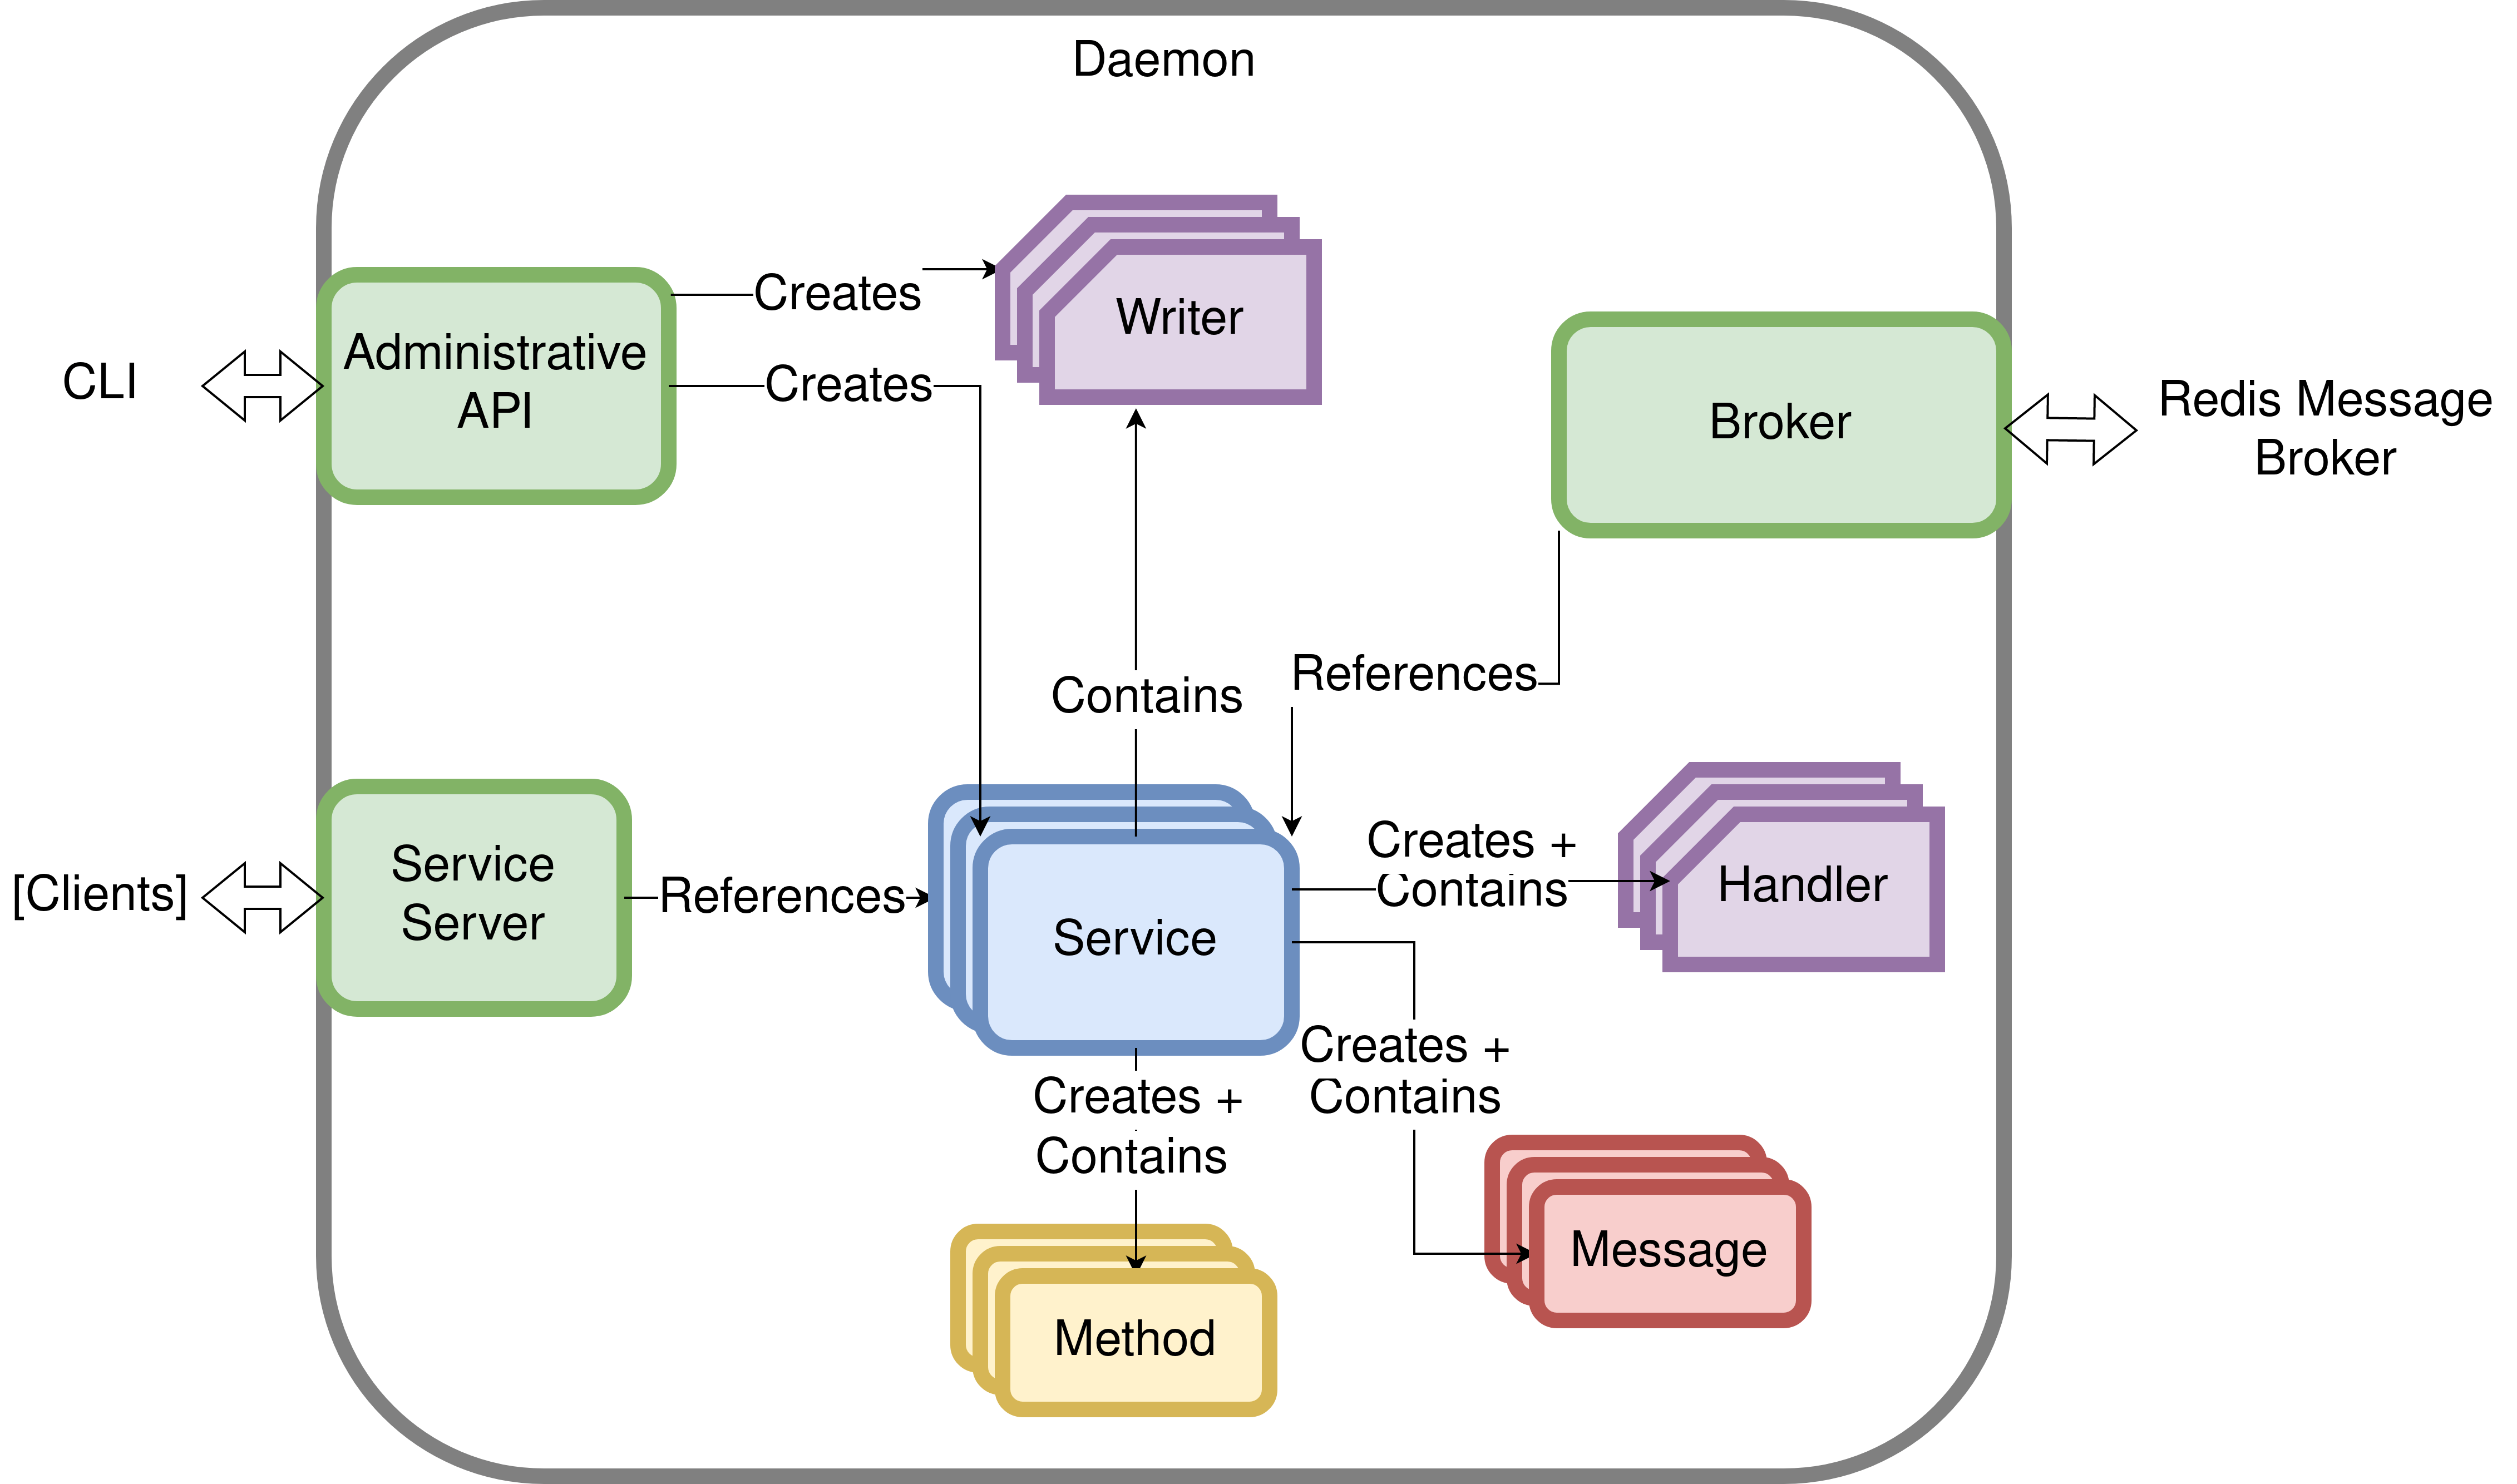
\includegraphics[width=\linewidth]{arch.png}
    \caption{Architectural overview of the daemon, describing how its components are created, referenced and stored in memory.}
\end{figure}
\section{Overview}
A single instance of the Pandit daemon will be run on each host in a cluster of machines. When a client queries
a service, the daemon will first check the cache for the data. If it cannot find it, it will delegate the request
to an authoritative container in the cluster.

Since the mapping between the data returned by the authoritative container and, the data returned by the gRPC service is
user-defined. Pandit provides options to annotate specific fields in return types to allow for the efficient caching of
common requests; greatly reducing the amount of queries that need to be sent to the authoritative container.

Each daemon will be responsible for handling all queries sent by clients on their node. As well as handling all queries sent to servers on their node.

When a query is received by a daemon, it first checks its local cache to ensure that the data has not been previously cached.

\begin{figure}[hbt!]
    \centering
    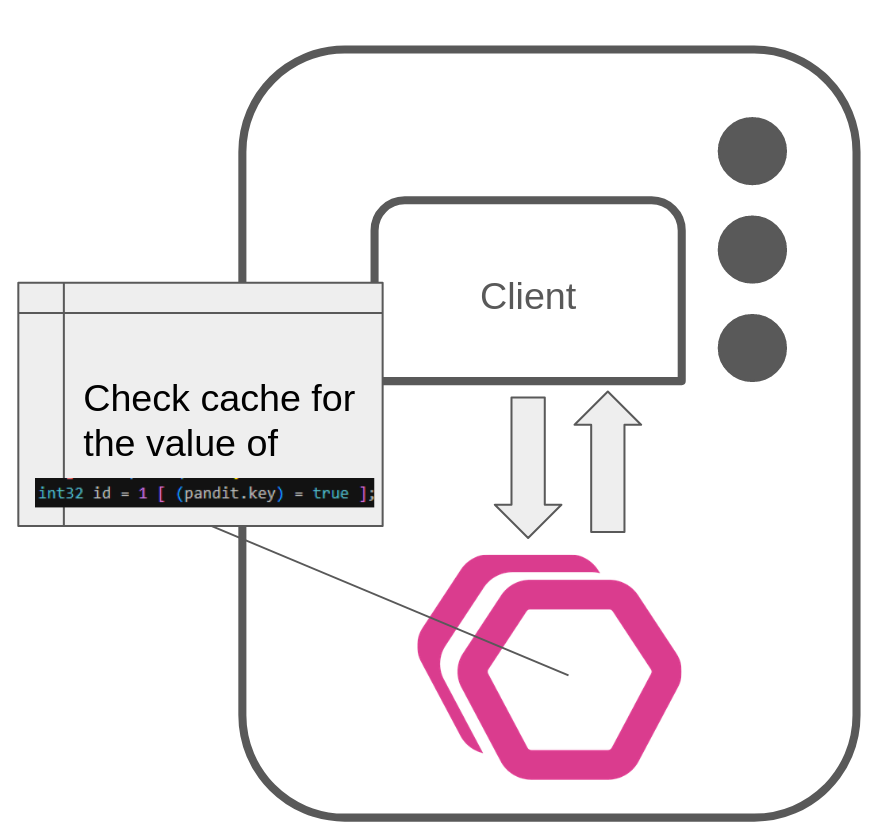
\includegraphics[width=\linewidth]{cache.png}
    \caption{Diagram of cache being looked up after a request is sent to the daemon}
    \label{fig:admin}
\end{figure}

If there is no cache hit, and the server that provides this data is on \textbf{another} node. The query will be delegated to the node in question.

\begin{figure}[hbt!]
    \centering
    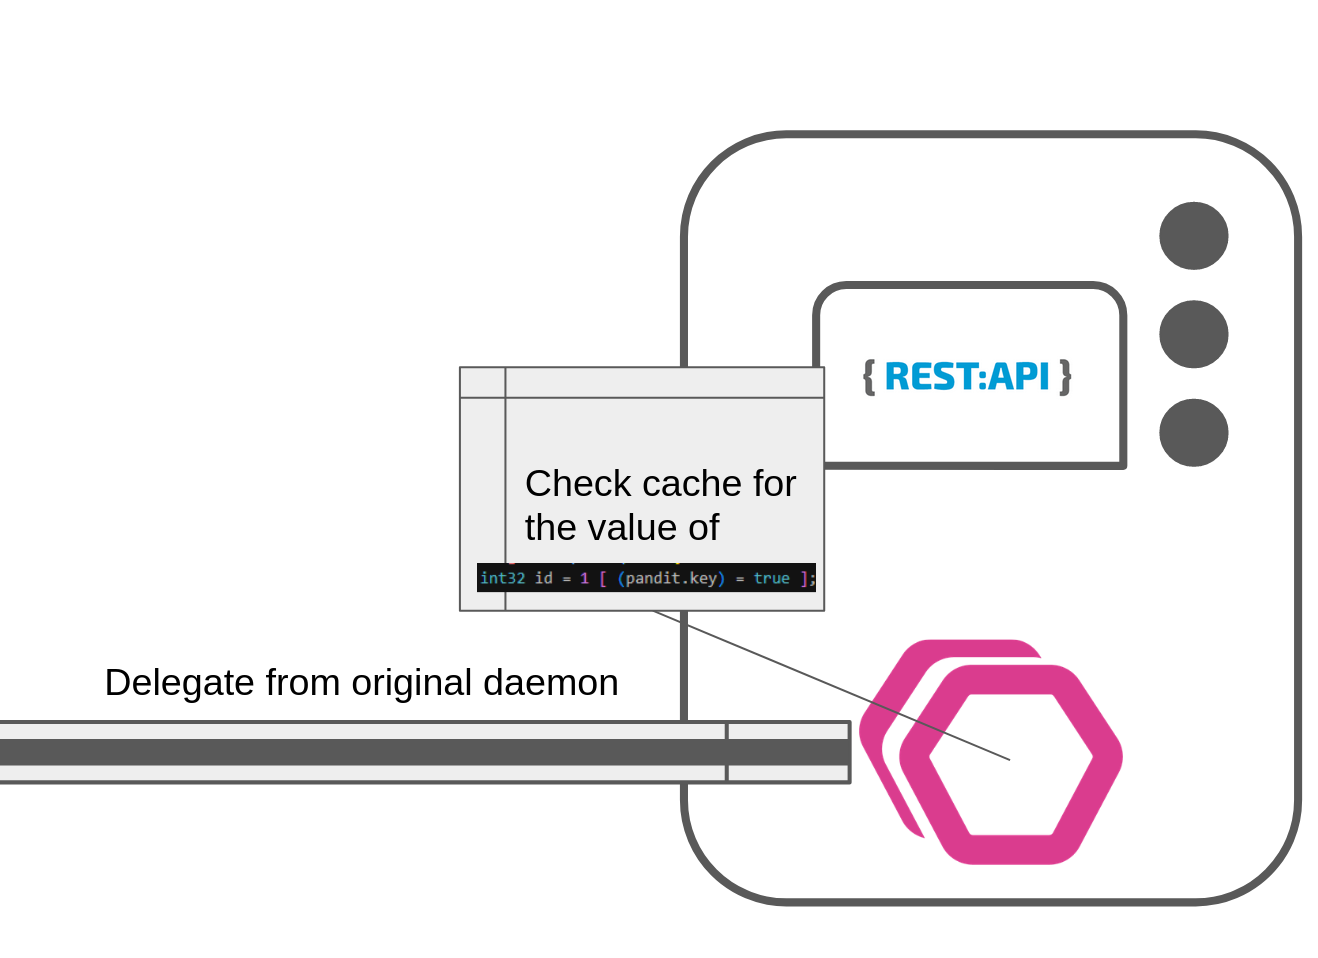
\includegraphics[width=\linewidth]{cache_del.png}
    \caption{Diagram of cache being looked up after a request is delegated from the original daemon to the daemon that is responsible for the application. In this case, a REST API.}
    \label{fig:admin}
\end{figure}

Each daemon maintains its own cache table, a delegated request can have a second chance of a chance of a cache hit.

If no cache hit occurs on the daemon that is responsible, the request will be translated and sent to the application.

\begin{figure}[hbt!]
    \centering
    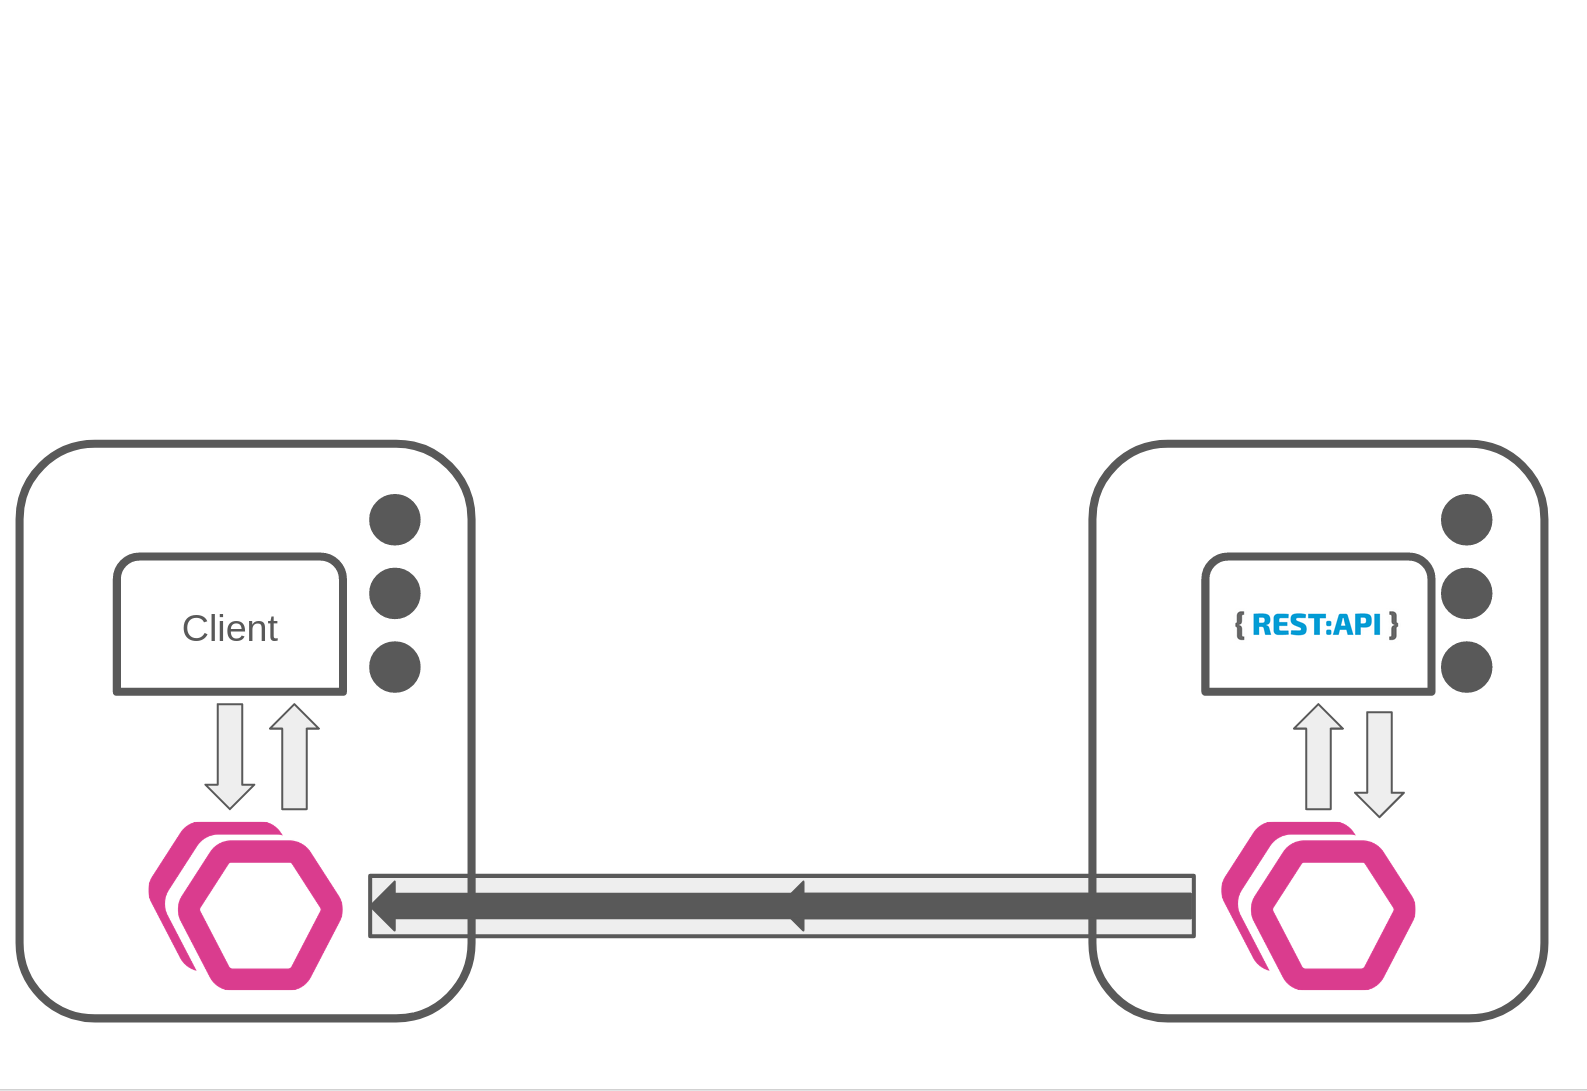
\includegraphics[width=\linewidth]{delegate.png}
    \caption{Diagram of a query being delegated from one daemon to another. Translating the request and sending it to the application. In this case, a REST API.}
    \label{fig:admin}
\end{figure}

\newpage

The daemon was implemented with the following components:

\section{Administration API}
\label{sec:api}
This is the API that is used to configure the daemon. It is a \nameref{sec:grpc} service that is exposed via a port on the loopback interface of each host.
A CLI client is used to interface with the API. Currently, the only supported method is to add a new \textit{\nameref{sec:service}} to the daemon.
This entails the following:
\begin{itemize}
    \item Creating a new \textit{\nameref{sec:service}} based on the parameters provided by the user.
          This includes providing Protobuf that was sent from the client as a byte array.
    \item Adding the service to the \textit{\nameref{sec:broker}}. The broker tells the other daemons about the service that this
          node is hosting the service in question.
    \item Adding the service to the \textit{\nameref{sec:server}} provides a generic gRPC Service for requests from clients.
\end{itemize}

The Proto file for the Administration API is the following:
\begin{lstlisting}
syntax = "proto3";

package api;

service API {
  rpc StartService(StartServiceRequest) returns (StartServiceReply) {}
}

message StartServiceRequest {
  string name = 1;
  bytes proto = 2;
  int32 port = 3;
  oneof container {
    string docker_id = 4;
    string k8s_pod = 5;
    string k8s_service = 6;
    string k8s_replica_set = 7;
    string k8s_stateful_set = 8;
  }
  bool delegated = 9;
}

message StartServiceReply {}
\end{lstlisting}

This is what the following fields in \textit{StartServiceRequest} represent:

\begin{itemize}
    \item \textbf{Name} - The unique identifier for the service. The identifier is used as the gRPC Service Name by clients querying the service.
    This is because multiple services can be run from the same Proto file; meaning there must be a unique identifier separate from the Proto file for each service.
    
    \item \textbf{Proto} - This is the \textbf{raw file bytes} of the Proto file. The reason why the entire Proto file is sent in the request, is that the CLI is responsible for managing the Proto files. While the daemon is responsible for parsing the Proto files.
    
    Storing the Proto files inside the requests allows for all the information necessary to start a service to be directly available inside the request. Making persistent storage of services much simpler to implement and maintain.
    
    \item \textbf{Port} - This is the Port that the application being proxied is exposed on. It is used to construct the address that the daemon will send traffic to for this particular service.
    
    \item \textbf{Container} - This is a set of optional fields that are used to deploy services in different \nameref{sec:deployment_modes}. 
    
    These will be covered in the \textit{\nameref{sec:deployment_modes}} section.
\end{itemize}

After the service is created and added to both the Broker and Server. The service must be stored in non-volatile storage for posterity.
Pandit daemons can be restarted and redeployed from time to time; Services added to the daemons must persist through this.

After adding a service, Pandit will serialise the raw \textit{StartServiceRequest} and save it to a uniquely named file in its current working directory.

Subsequently, when Pandit starts up, it will look for services in the Current Working Directory. If some are found, they will be sent directly to the \textit{StartService} gRPC method, being added to the local daemon.

\begin{figure}[hbt!]
    \centering
    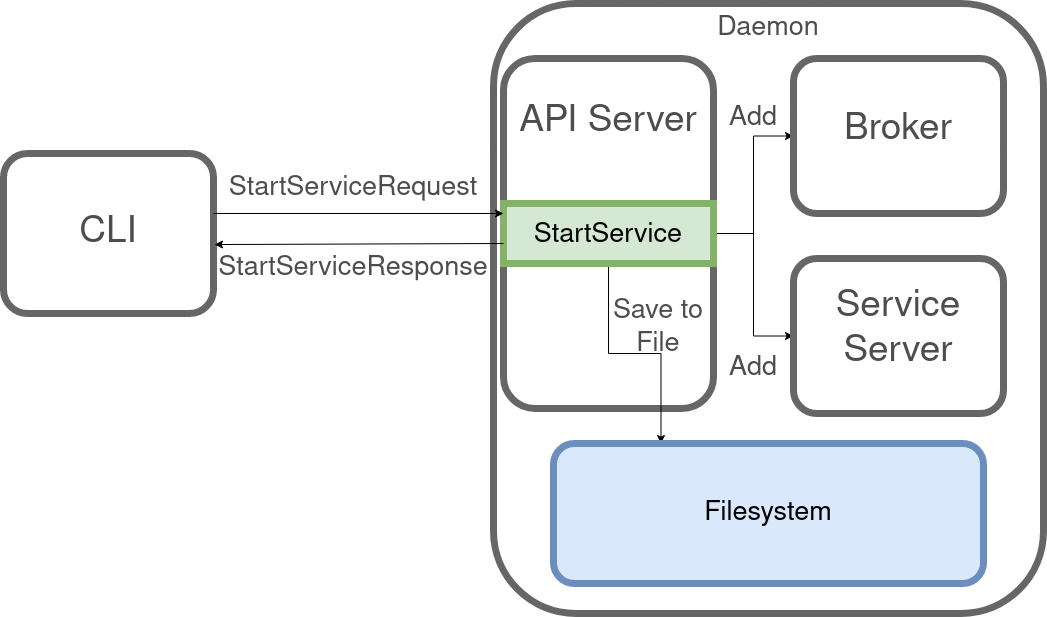
\includegraphics[width=\linewidth]{admin.png}
    \caption{Diagram of AddService being called by the CLI and sent to the Administration API}
    \label{fig:admin}
\end{figure}

\section{Service}
\label{sec:service}
This is a \textit{struct} that represents a service that is hosted by the daemon. It is created by the \textit{\nameref{sec:api}} and
takes in a Protobuf specification.

The constructor parses the provided Proto specification, and builds an in-memory mapping of all methods, messages, and their fields.
This includes parsing user defined options imported from the \textit{pandit package}.

Here are the options available to the user in \textit{pandit.proto}:

\begin{lstlisting}
syntax = "proto3";
import "google/protobuf/descriptor.proto";

package pandit;

message CacheOptions {
  bool disable = 60031;
  uint64 cache_time = 60032;
}

extend google.protobuf.FieldOptions {
  string absolute_path = 50020;
  string relative_path = 50021;
  CacheOptions field_cache = 50036;
  bool key = 50037;
}

extend google.protobuf.MessageOptions { string path = 50030; }

extend google.protobuf.MethodOptions { CacheOptions cache = 50034; }

extend google.protobuf.ServiceOptions {
  string name = 50010;
  CacheOptions default_cache = 50035;
}
\end{lstlisting}

This is what the options are used for:
\begin{itemize}
    \item \textbf{Cache Options} - This defines the \textit{caching strategy} for particular Messages, Fields and Services. 
    
    It contains the field \textbf{disable}, which when set to true disables the caching of the resource. The field \textbf{cache$\_$time} defines the amount of time this revision of the cache should be stored for before being invalidated. If neither field is set, the cache will persist permanently.
    
    \item \textbf{Key} - The primary key of a message - The key is required to be put on \textit{exactly one} field in each input message. The reason for this is twofold:
    \begin{enumerate}
        \item It is required to build out the cache table on each daemon. The value of the primary key is serialised and used to index the cache; per particular method on a daemon.
        \item It may be used in the translation between the Protocol Buffer and the desired format. For example, SQL requires a primary key for many commands.
    \end{enumerate}
    
    \item \textbf{Name} - The name of the service - In lieu of the name of the Service defined in the Proto file. A custom name can be used to identity the gRPC service by using this custom option.
    \item \textbf{Path} - This defines the path of a message in an abstract representation parsed from the response from the proxied application.
    
    This is used in situations where the required data in a JSON field is actually a sub-object of the root object provided.
    
    For example, take this JSON response:
    \begin{lstlisting}
    {
        "object": {
            ...
        }
    }
    \end{lstlisting}
    If you wanted your output message to be parsed from the \textit{object} field instead of the root object. You would define your message as the following:
    \begin{lstlisting}
    message ExampleResponse {
        option (pandit.path) = ".object";
        int32 id = 1;
        string user = 2;
    }
    \end{lstlisting}
    
    This is parsed via an abstract representation of the structured data, and so is not format-specific.
    The format of the path string is based on \textit{jq's parsing language} \cite{jq}. It is also designed to be able to parse any structured data format, that has been implemented inside Pandit. Not just limited to only JSON.
    
    
    \item \textbf{Absolute Path} - This defines the path of a field in a message; like in the message option \textbf{Path}. It uses a parsing language to define the path. In this case, however, it defines the path from the base object to the specific field that should be mapped.
    
    \item \textbf{Relative Path} - Like the \textbf{Absolute Path}. Defines a mapping between a field in the  abstract representation of the structured data, and the output message. In this case, the root object is assumed to be the message that the field is defined in. 
    
    Take the following example:
    \begin{lstlisting}
    message ExampleResponse {
        option (pandit.path) = ".object";
        int32 id = 1; [(pandit.relative_path) = ".user.id"]
        string user = 2;
    }
    \end{lstlisting}
    
    In this case, the field user would be mapped to the path \textit{.object.user.id} in the abstract representation of the structured data.
\end{itemize}

\subsection{Sending Data to the Host}

The primary use case of the service is to proxy an application. 
Thus, the service provides a method used to provide data to the application.

Firstly, it translates the request using a method on the Handler called \textit{ToPayload}, to the required format for the application being proxied.

It then passes the translated request payload, as well as the \textit{\nameref{sec:handler}} for the specific method, to a \textit{\nameref{sec:writer}}. 
The writer then sends the request to the proxied application. With the \textit{FromPayload} method on the handler, it then parses 
and returns the response.

The service struct handles the calling of the writer and handler. This is due to it containing all the necessary data to call the methods on these traits.

\begin{figure}[hbt!]
    \centering
    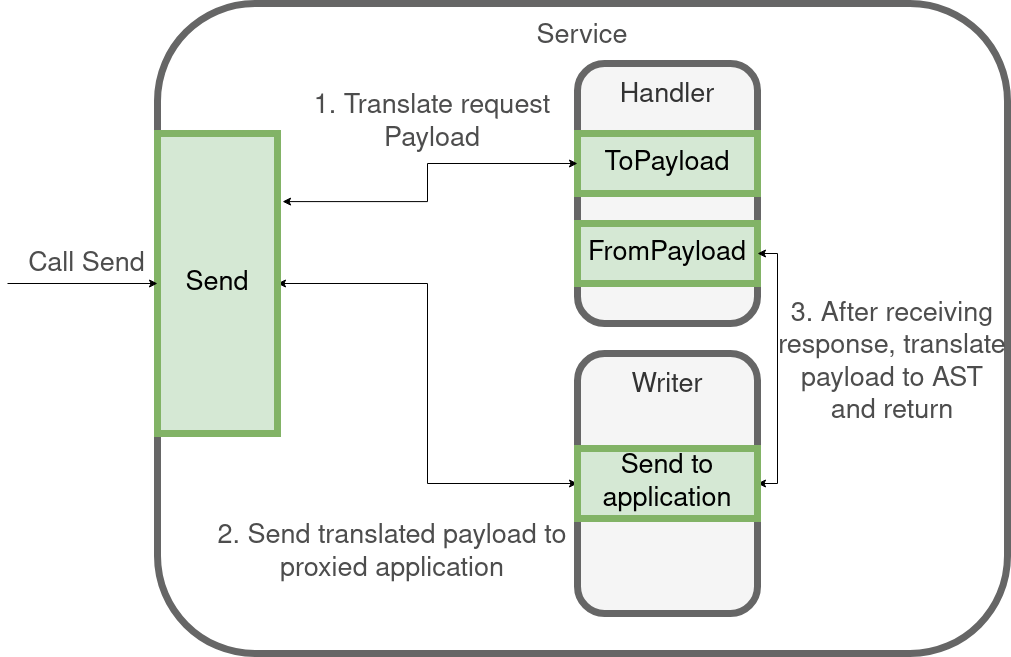
\includegraphics[width=\linewidth]{Service.png}
    \caption{A Diagram explaining how the Service sends a payload to the proxied application.}
    \label{fig:admin}
\end{figure}

\newpage

\section{Message}
\label{sec:messages}
Pandit stores an abstract representation of the gRPC messages used by Service's methods.
It contains the following fields:

\begin{itemize}
    \item The message name.
    \item The path of the message - Used during the aforementioned translation stage. Used to parse a returned payload that has the necessary data inside a field.
    \item Fields - This contains a map of all the fields defined in the Proto message.
    \item Message - This contains metadata such as options defined inside the Proto message.
\end{itemize}

The primary purpose of the Pandit Message is to provide the methods used to convert a Protocol Buffer payload to an Abstract Representation called \textit{Fields} and vice-versa.

\begin{figure}[hbt!]
    \centering
    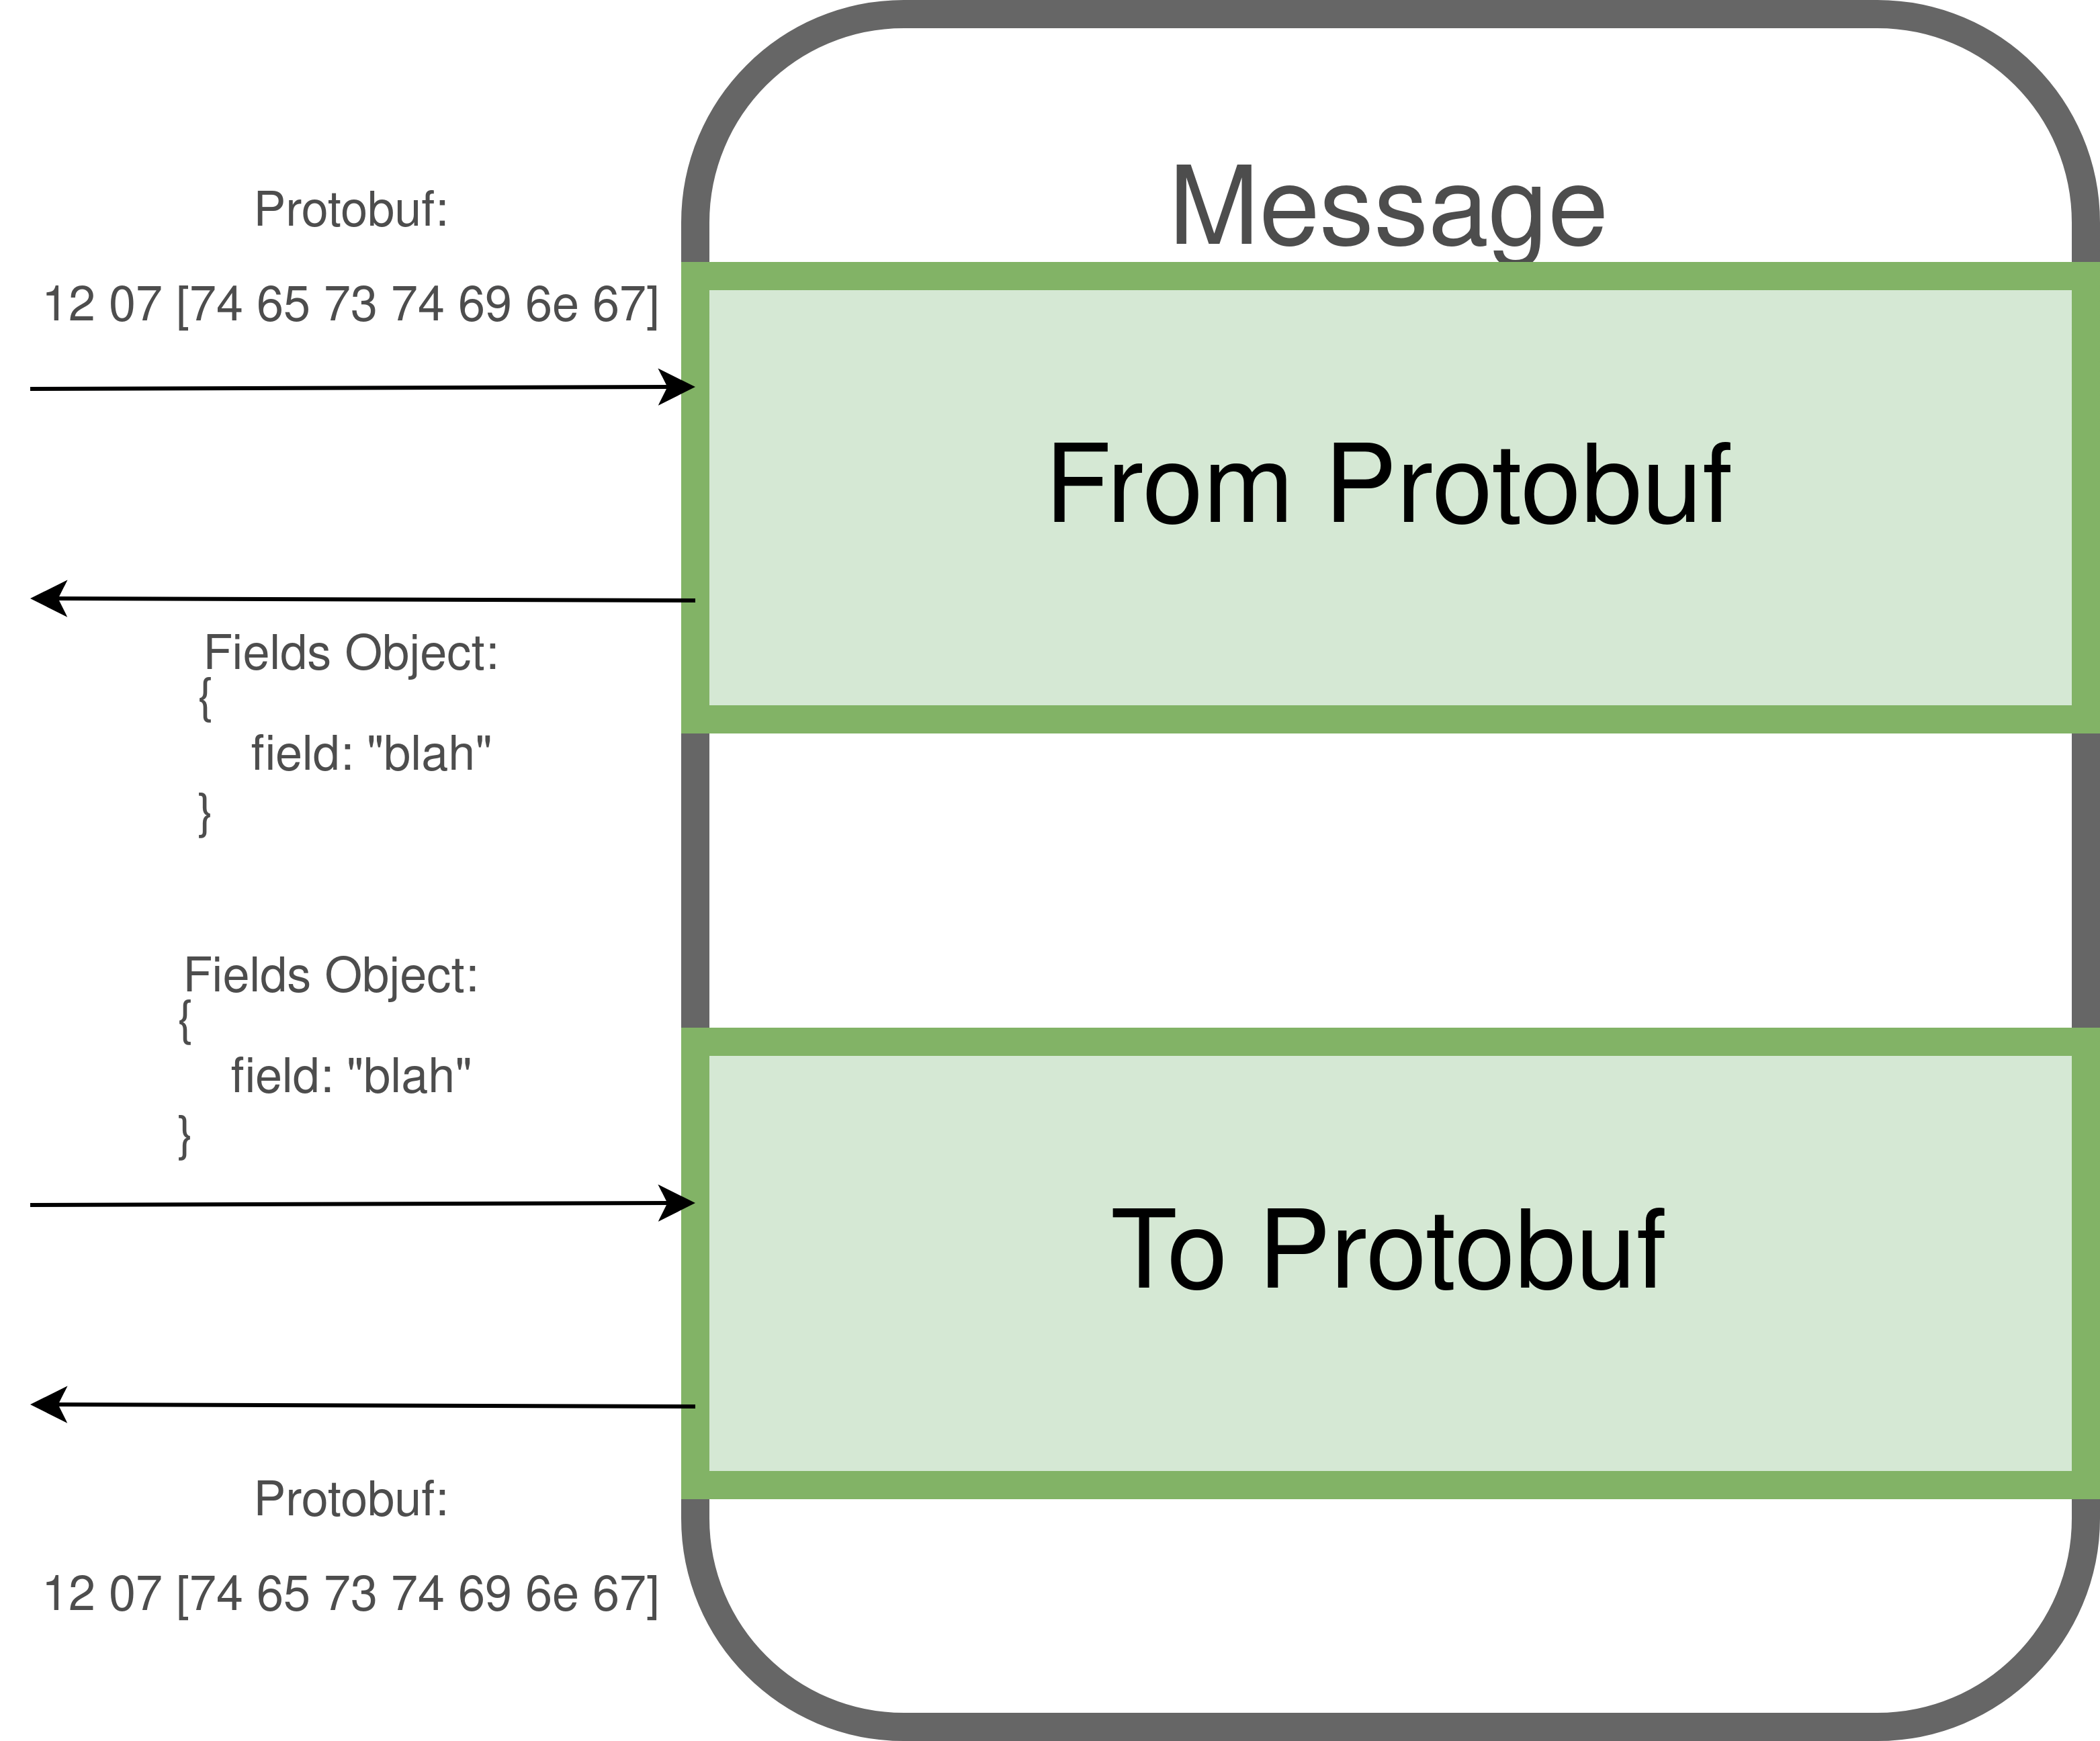
\includegraphics[width=\linewidth]{Message.png}
    \caption{A Diagram of the public methods available on the Message struct}
    \label{fig:admin}
\end{figure}

\section{Method}
\label{sec:methods}
This represents a Protocol Buffer Method. A Method is defined by an input \nameref{sec:messages} and an Output Message. It will only contain two instances of this struct.

The Pandit method contains the following:

\begin{itemize}
    \item All the Proto options users have set on the particular gRPC method.
    \item The \nameref{sec:handler} for this particular method.
    \item The input (parameters) and output (returned) messages.
    \item The primary key parsed from the input message. This will be used for building a cache table on the local daemon.
\end{itemize}

\section{Writer}
\label{sec:writer}
This is a trait \cite{trait} that represents a way of sending a query to the authoritative container.
It takes in abstract representations of the Protocol Buffer Message called \textit{Pandit \nameref{sec:messages}s} and a \textit{\nameref{sec:handler}}.
The writer uses the \textit{\nameref{sec:handler}} to convert the data to a bytes array.
It then constructs a full request in the format required with the payload from the handler. It does this by encapsulating the payload with the required headers.

For example, the Handler could return a JSON payload. The writer would then encapsulate the payload in a series of HTTP headers. This approach is designed to be implemented for any format, for example, SQL.
Finally, it then sends the request to the authoritative container.

\begin{figure}[hbt!]
    \centering
    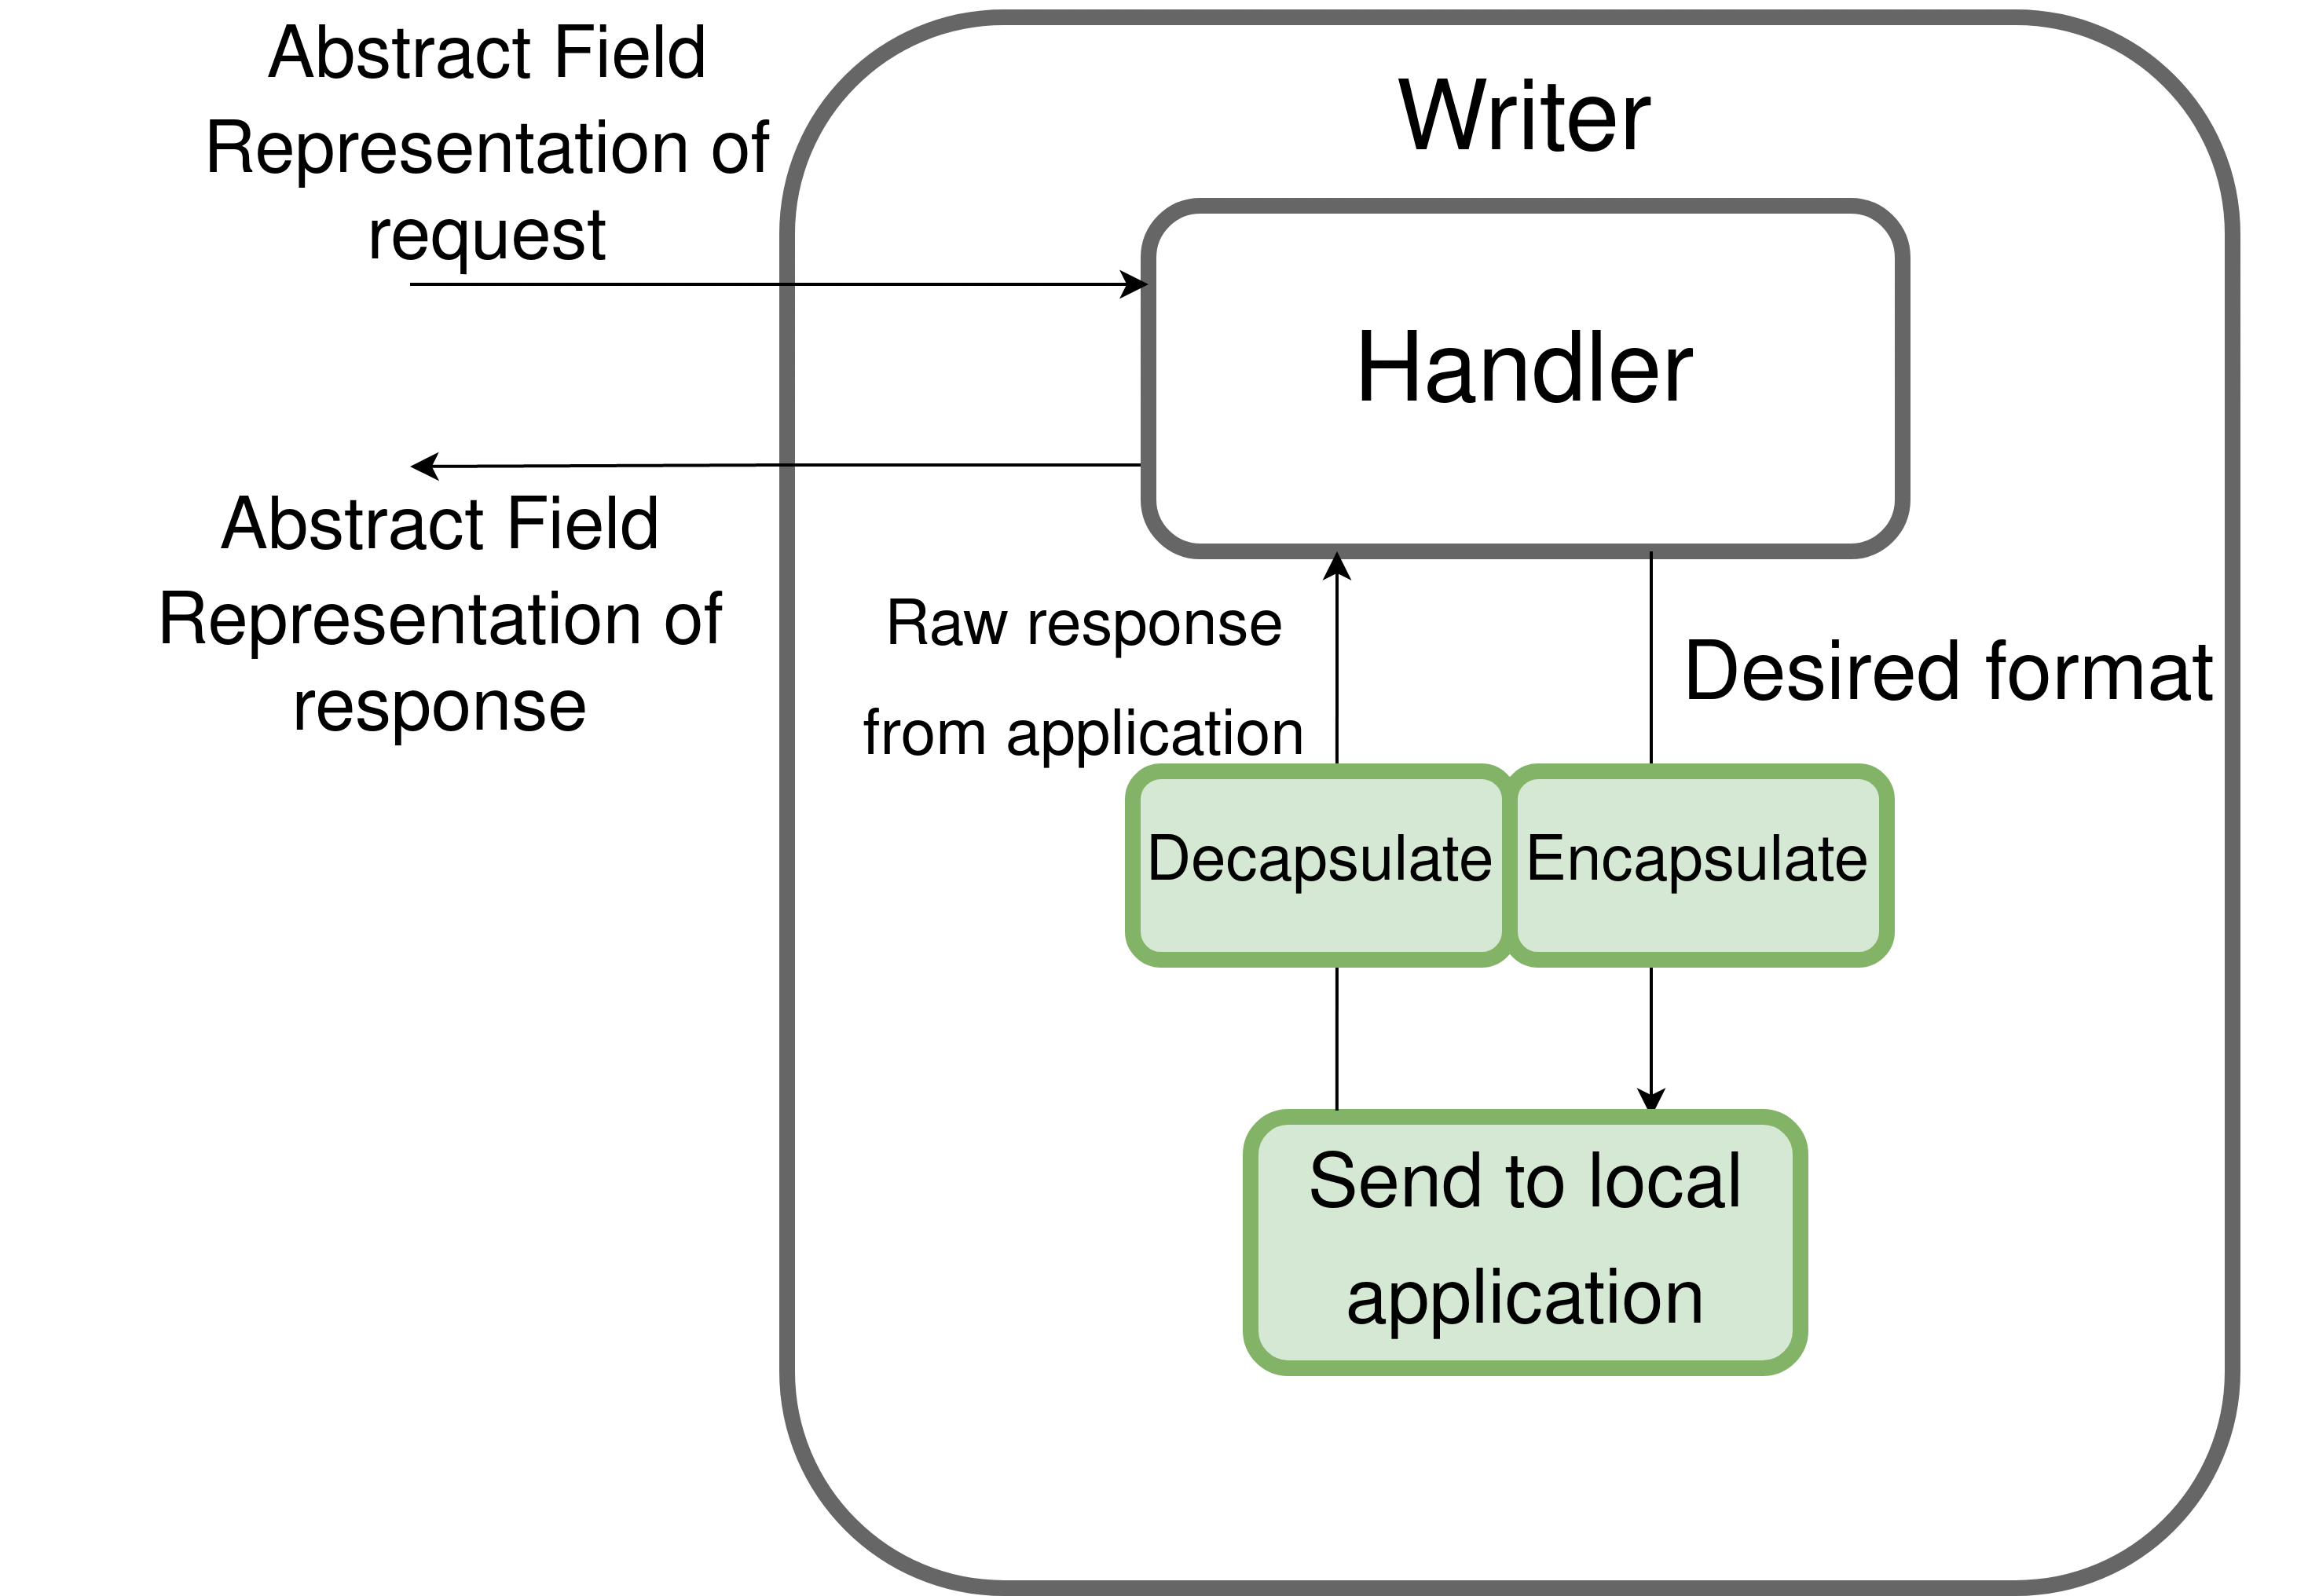
\includegraphics[width=\linewidth]{writer.png}
    \caption{A Diagram of the writer communicating with the local application}
    \label{fig:admin}
\end{figure}

\newpage
\section{Handler}
\label{sec:handler}
The \textit{\nameref{sec:handler}} is used to convert to, and from, the abstract fields representation of the data provided to the writer.

The Handler is a trait (an interface) that provides the following methods:

\begin{itemize}
    \item \textbf{To Payload} - This takes in an abstract field representation parsed from the gRPC request. Through the relevant Pandit \nameref{sec:messages}, converts it into the desired payload that should be sent to the server.
    \item \textbf{From Payload} - This takes in a buffer of bytes containing the decapsulated payload received from the proxied application. Then converts it into the abstract field representation.
\end{itemize}

\section{Broker}
\label{sec:broker}

The Broker is the glue that allows the daemon to be aware of, and communicate with, other daemons in the cluster.
The broker interfaces with a Redis \cite{redis} instance. The instance is connected to all the daemons to facilitate this.

The reason behind Redis being chosen is as follows. Other message brokers \cite{broker} such as Kafka had Rust libraries that were less documented and maintained. 
In comparison, Redis has an easy to use, well documented Rust library. It also provided all the features Pandit required of a message broker.

The Redis instance can be deployed in any manner. Just as long as it exposes its API to each daemon.

When constructing the broker, the user provides the address of the Redis instance. It will maintain a connection to the Redis instance for the entirety of the run time.

The broker will maintain a connection to Redis's PUB/SUB \cite{pubsub} throughout the lifetime of the program. It will listen for updates to subscribed topics, such as cache updates to subscribed services.

It provides many methods to interact with the Redis instance:
\begin{itemize}
    \item To add a new \textit{\nameref{sec:service}} to the broker. 
    
    This will send information to Redis such as:
    
    \begin{itemize}
        \item The cache options that were set.
        \item The address of the current daemon. This will allow other daemons to look up the name of the service, and find the address of the daemon that's responsible for it.
        \item The methods this service has. This includes a serialised version of the entire \nameref{sec:methods} struct.
        \item The input and output messages for each method. This includes a serialised version of the entire \nameref{sec:messages} struct.
    \end{itemize}
    
    \item To query the broker for the address of the daemon responsible for a \textit{\nameref{sec:service}}.
    This will look up the value that was set by the "add service" method.
    
    \item To subscribe to cache updates for a particular method. This will be updated in a listener thread that subscribes to Redis's PUB/SUB feature.
    
    \item To publish new cache to all interested daemons in the cluster. This will send a serialised version of the necessary data to said daemons.
    
    \begin{figure}[hbt!]
        \centering
        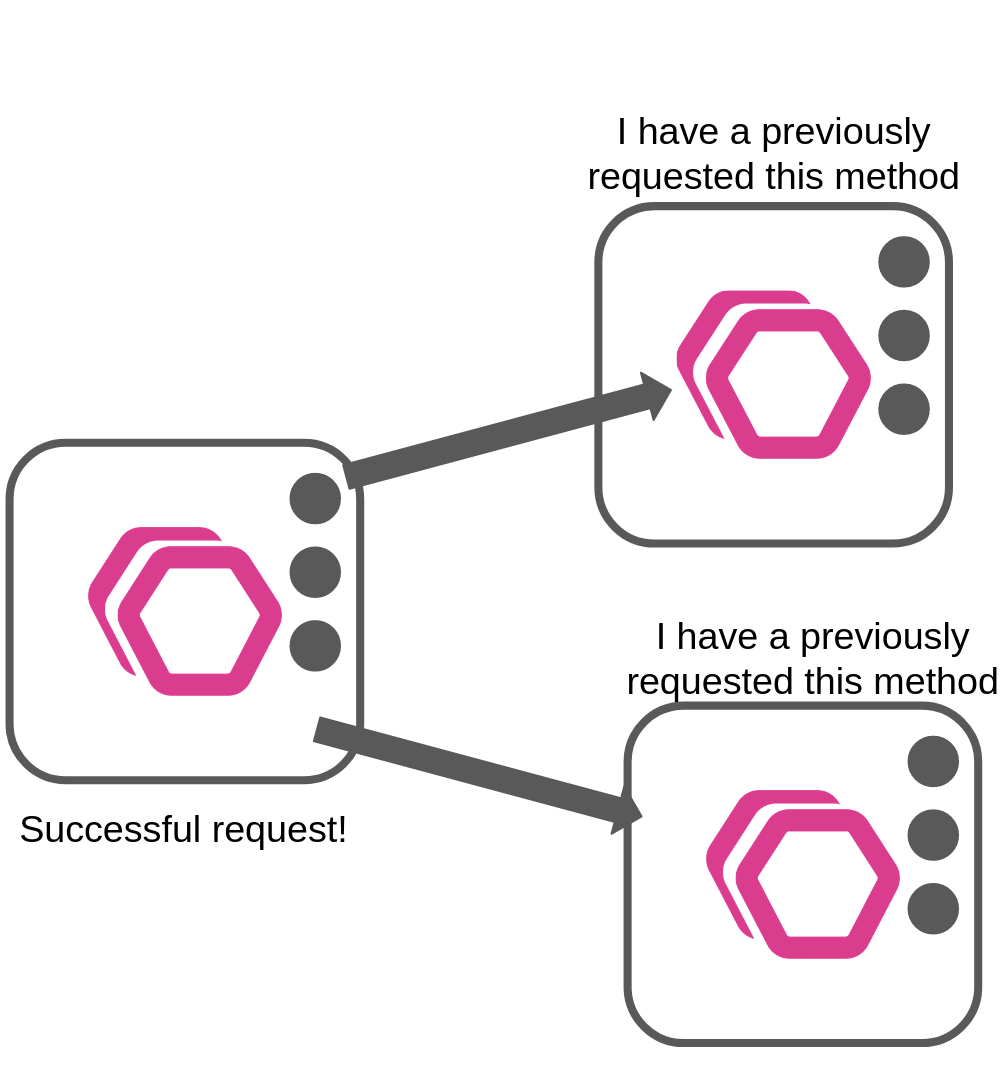
\includegraphics[width=\linewidth]{pubsub.png}
        \caption{A Diagram of cache subscription from the perspective of the daemons that are subscribed}
        \label{fig:admin}
    \end{figure}
    
    \newpage
    
    \item To check if there is a cache hit locally for a particular query. This will read from a local table. The table is updated automatically via the Redis PUB/SUB functionality.
\end{itemize}


\section{Service Server}
\label{sec:server}
This provides a custom gRPC service handler. It is responsible for handling all requests from clients on the host it's running on.
When a gRPC request is received, it will parse the service and method name from the request.
It will first check the cache for the data based on this information. If it cannot find it,
it will delegate the request to the \textit{\nameref{sec:service}}.

However, the \textit{\nameref{sec:service}} may not be available on the current host. In this case, the request will be delegated to the host that the
service is available on. The host is found by querying the \textit{\nameref{sec:broker}} for the address of the host the service is on.
After a response is received, it will publish the data to the cache using the \textit{\nameref{sec:broker}}.

It will also check with the broker to ensure that if the daemon hasn't subscribed to the cache for this method, it must do so.

\begin{figure}[hbt!]
    \centering
    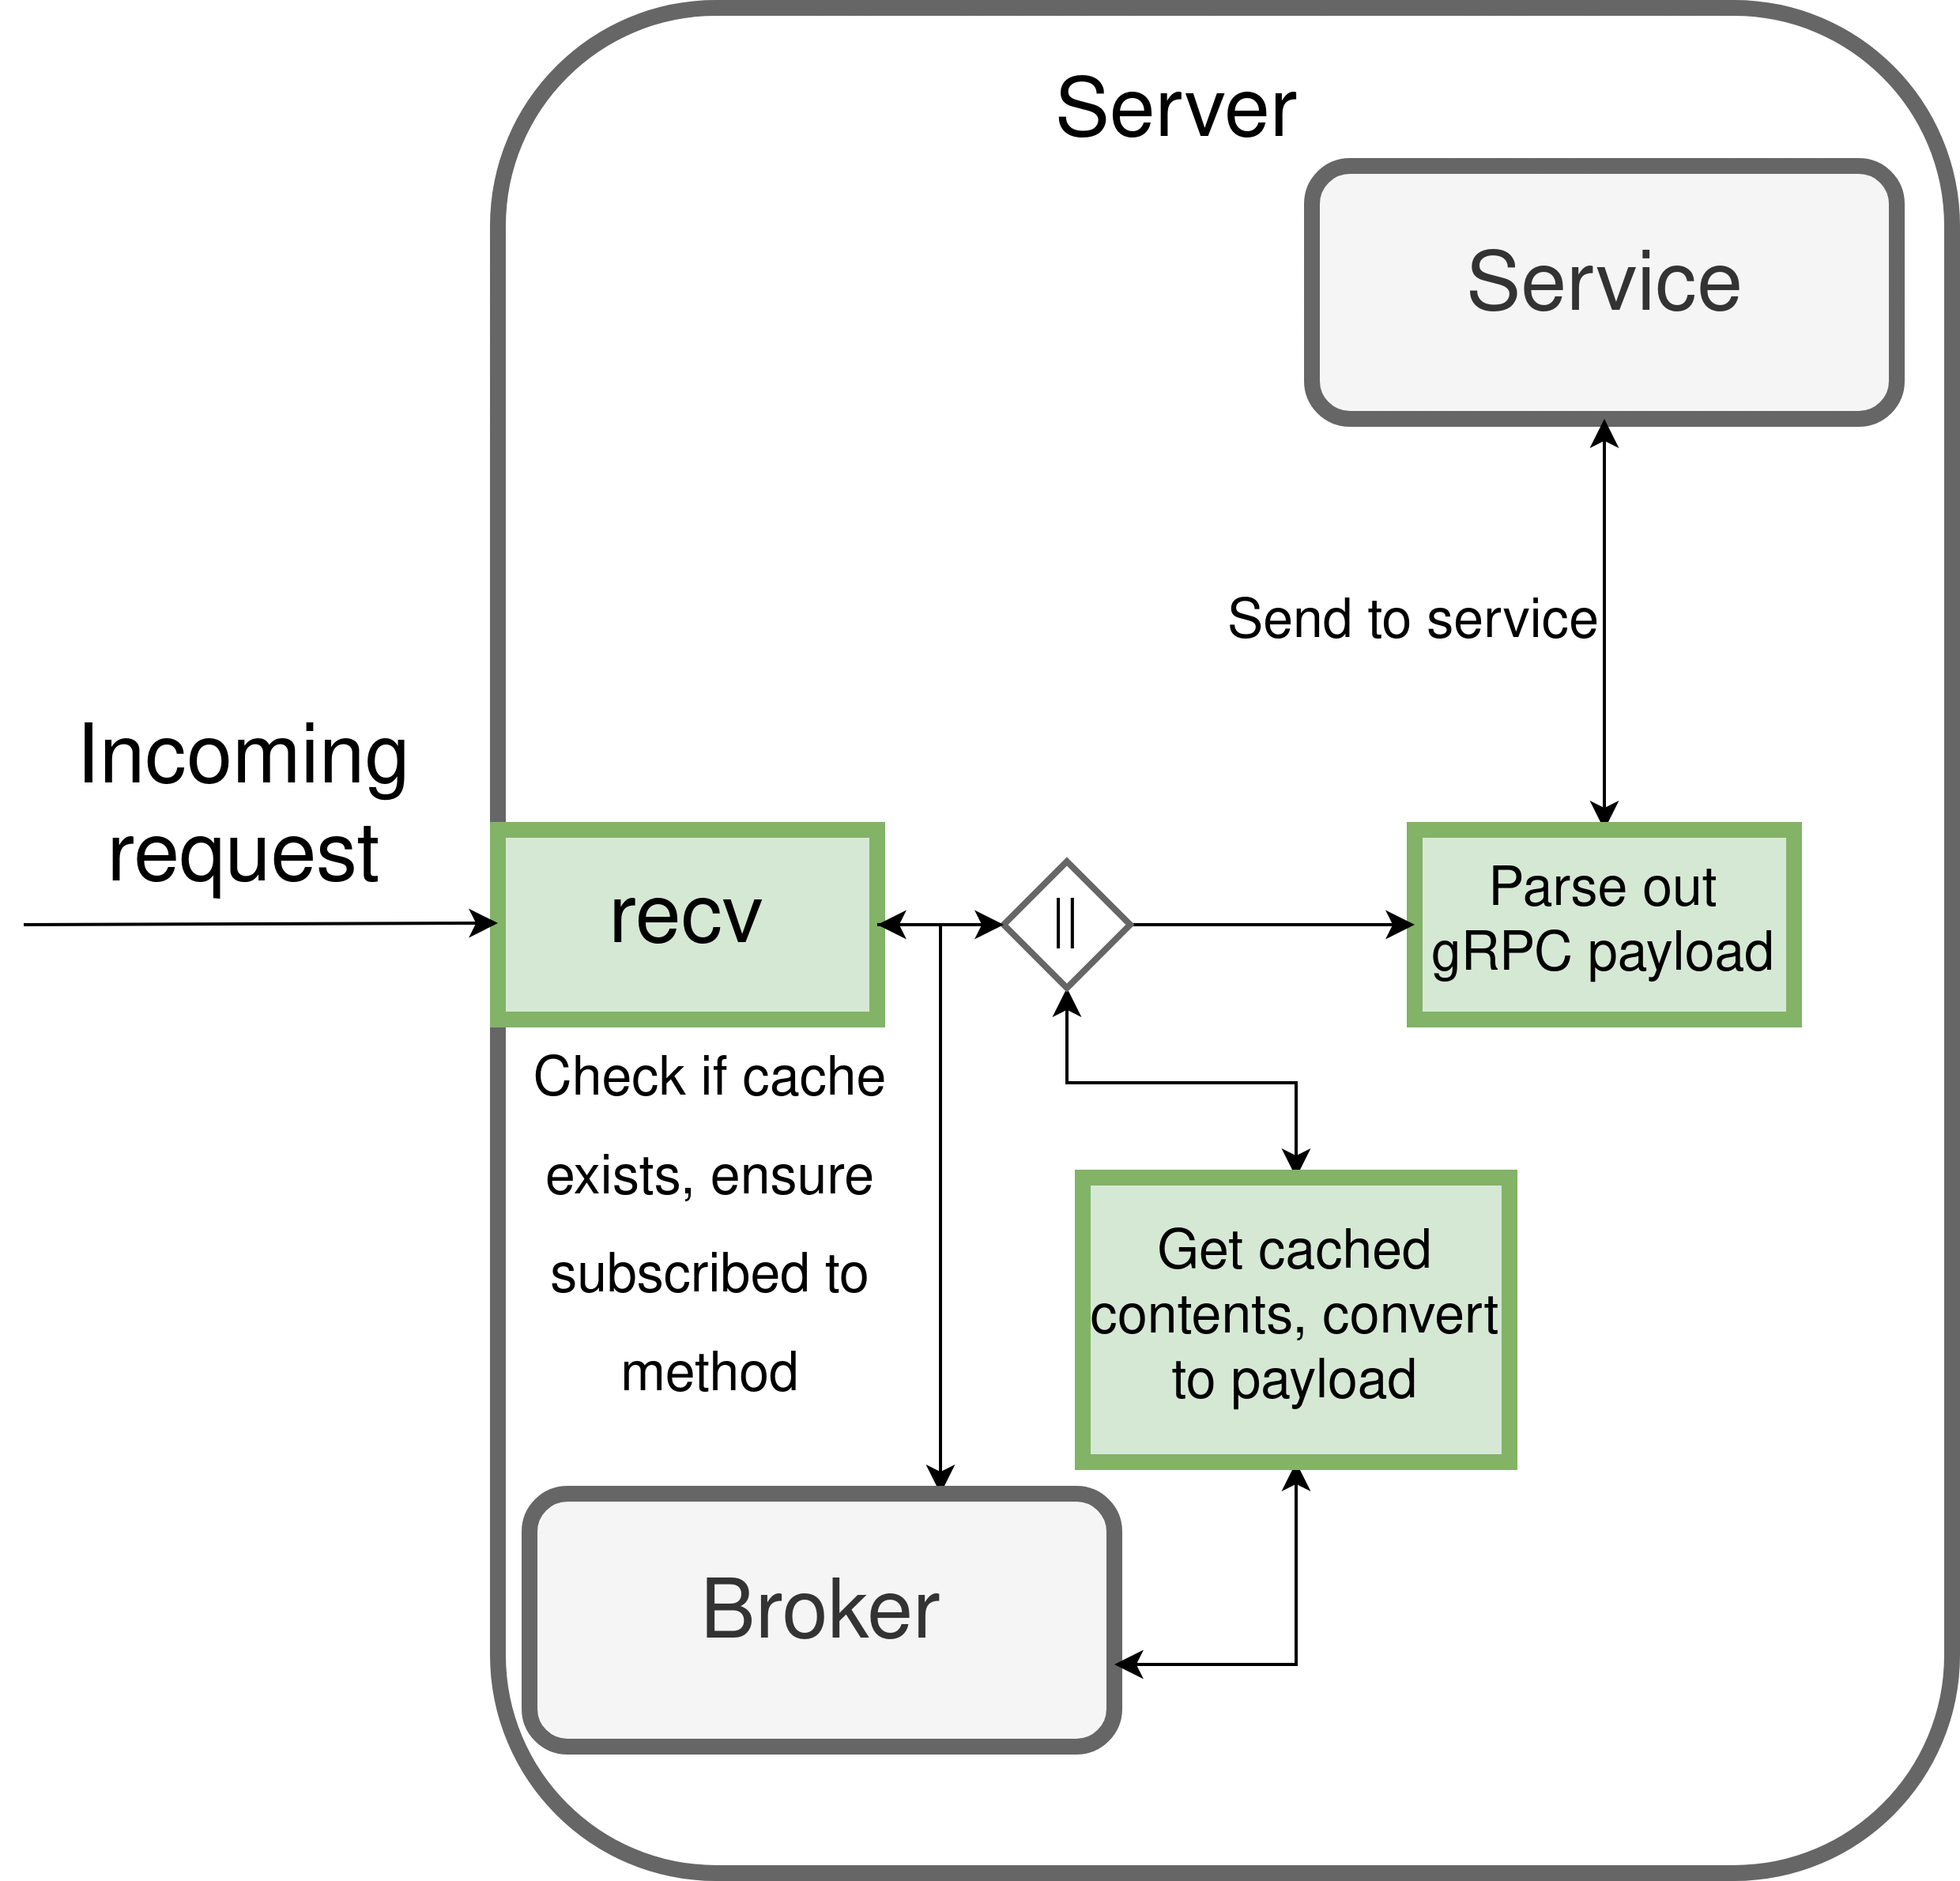
\includegraphics[width=\linewidth]{server.png}
    \caption{A Diagram of the operation service server.}
    \label{fig:admin}
\end{figure}

\newpage

\section{The CLI}
\label{sec:cli}
The CLI provides a command line interface to configure the daemon.
It imports the gRPC client library that was generated by the Protobuf compiler. The CLI uses the client to interface with the daemon's \textit{\nameref{sec:api}}.

It runs as a standalone binary. By default, it connects to the daemon via a known port on \textit{localhost}. 
However, a flag called \textit{--daemon-address} can be passed to modify the address it will connect to.


\begin{figure}[hbt!]
    \centering
    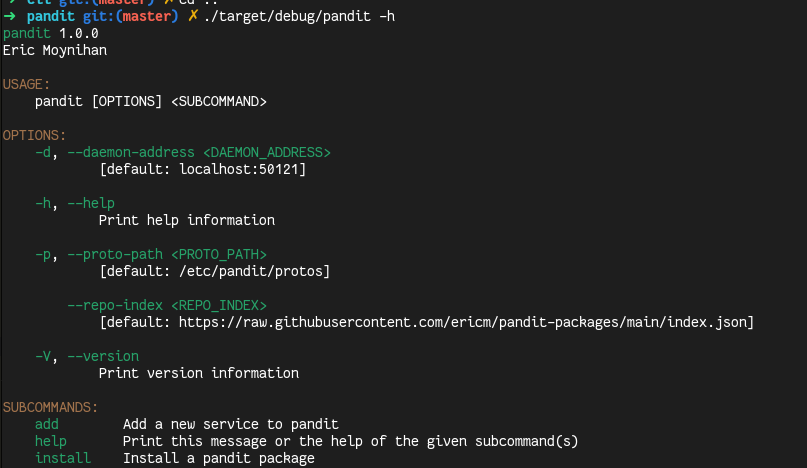
\includegraphics[width=\linewidth]{cli1.png}
    \caption{A screenshot of the help menu from the CLI.}
    \label{fig:admin}
\end{figure}

\newpage

It supports the following commands:

\begin{itemize}
    \item \textbf{Add} a new service to pandit - This will take in a path to a \textit{Pandit file}.
    
    This is a TOML file that defines how the service should be run. It includes fields such as the name of the service, the proto file that should be used, (which is found in the path pointed to by the \textit{--proto-path} flag) and the port that the application is exposed on.
    
    \begin{figure}[hbt!]
        \centering
        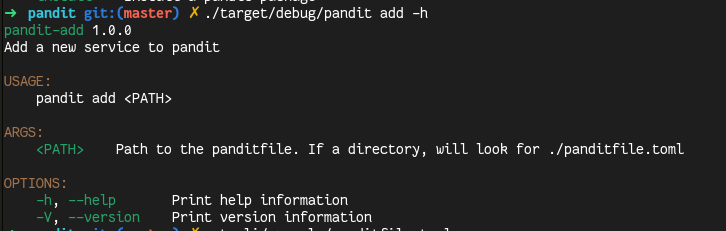
\includegraphics[width=\linewidth]{cli2.png}
        \caption{A screenshot of the help menu for the \textit{add} command from the CLI.}
        \label{fig:admin}
    \end{figure}
    \newpage
    
    \item \textbf{Install} a Proto file. In this context, we'll call it a \textit{package} due to it containing extra metadata.
    
    This is achieved by:
    
    \begin{enumerate}
        \item Check a centralised repository for a list of available services.
        \item Based on the name provided to the command, get information from the repository on the Proto file. This includes:
        \begin{itemize}
            \item The version of the package.
            \item The URL to the Proto file.
            \item A URL to the README (for display purposes, unused during installation).
            \item A URL an image/logo (for display purposes, unused during installation).
            \item An optional "image". This is either a link to a Docker Image \cite{image} for Docker or a Helm Chart \cite{helm} for Kubernetes.
        \end{itemize}
        \item Install the "image" to the system if present.
        \item Download the Proto file to the path set by \textit{--proto-path} (by default it will be \textit{/etc/pandit/protos}).
    \end{enumerate}
    
    \begin{figure}[hbt!]
        \centering
        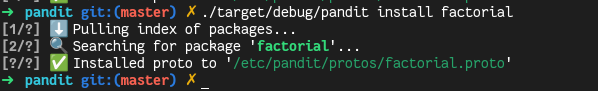
\includegraphics[width=\linewidth]{cli3.png}
        \caption{A screenshot of the installation succeeding for a package via the CLI.}
        \label{fig:admin}
    \end{figure}
    \newpage

\end{itemize}

\section{Deployment Modes}
\label{sec:deployment_modes}
Pandit is designed to be deployed within pre-existing infrastructure. Meaning, it needs to be able to be easily deployed in different types of 
distributed environments.


\subsection{Basic Deployment Mode}
This mode allows Pandit to be deployed on a set of servers that have network connectivity. A single Pandit daemon is deployed by the System Administrators on each server. They are then all configured to connect to a Redis endpoint. This allows the servers to communicate information on the services running on each server.

Services are added by running a command on the CLI. The service options available in this mode will be:

\begin{itemize}
    \item \textbf{Name} - Used to identify the service.
    \item \textbf{Proto} - The name of the Proto file installed on the system. Used to define the interface and translation method for the service.
    \item \textbf{Port} - Used to identify the network socket the daemon should connect to. In order to communicate with the application.
\end{itemize}

\subsection{Docker Deployment Mode}
\subsubsection{Background}
\textbf{Docker} is a platform used to deploy containerised applications. It runs as a daemon on a machine. It provides an API to manage
containers in runtime. Docker is used to isolate single applications using Linux kernel features such as cgroups. Cgroups allow for CPU, memory, disk and network isolation for a collection of processes.

This process is known as containerisation. Docker containers are deployed by providing Docker an Image. A snapshot of the filesystem is passed in to the running process; it contains all the dependencies it requires.

Docker gives each container its own IP address by default. This allows applications on the host machine to interface with the processes in containers via a bridge network. This also provides inter-container network connectivity.

Docker provides resources called 'volumes' to running containers. These come in three types: 

\begin{itemize}
    \item \textbf{Bind Mounts} - Maps between paths on the container's filesystem and the host's filesystem.
    \item \textbf{Docker Volumes} - Maps between a persistent storage resource managed by docker and a path on the container's filesystem
    \item \textbf{\textit{tmpfs} Mounts} - Provides a volatile in-memory filesystem to a path on the container's filesystem.
\end{itemize}

Docker also provides a 'network' resource that allows containers' networks to be bridged together. By default, containers are all added to the 'default' network. However, they can be configured to be connected to custom docker networks. Custom networks allow for selective isolation of network connectivity between containers.

Docker's API allows users and applications to query information about running containers. Including its IP address, the ports it has exposed and the image it's based on. It also allows resources such as containers and networks to be programmatically created. Docker's API is accessible on the host system via a Unix Socket, which provides an HTTP API that can be queried via docker's provided CLI or programmatically.

\subsubsection{Design}
Pandit in this deployment mode runs is designed to be run in a Docker container. It's aware that it's in a docker environment because it has been started with the command line argument \textit{--docker}. The container will be given a \textit{Bind Mount} to the Docker API's \textit{Unix Socket}. The bind mount allows access to the Docker API inside the container.

Pandit's Service deployment configuration specification includes the following additional option when Docker Deployment Mode is enabled:
\begin{itemize}
    \item \textbf{Container ID} - A unique ID used by Docker to identify a container on the system.
\end{itemize}

When a service is added, Pandit queries the Docker API for a container matching the provided container ID. 
If found, Pandit will do the following:

\begin{itemize}
    \item It will create a Docker network specifically to facilitate communication between Pandit, and the application.
    \item It will add both Pandit's container, and the application's container, to the network. Both of them will be assigned an IP address.
\end{itemize}

Pandit will then construct an address to be associated with the \textit{\nameref{sec:service}}. It uses the IP address and port received during construction to achieve this.

When Pandit must query the application in the future, it will use this address to do so.

Clients can query Pandit in a number of ways:

\begin{itemize}
    \item They can be deployed in Docker, and interface with Pandit via a bridge network.
    \item They can be running outside of Docker. Pandit's gRPC API port can be exposed on the host system through Docker configuration. The client can then interface with Pandit via this port.
\end{itemize}

\subsubsection{Multiple Hosts}
When dealing with multiple hosts running separate Docker systems. A Redis instance will be deployed on one of the hosts. It will be exposed via a port forwarding. Pandit's APIs on all hosts will also be port forwarded. 

During deployment, each instance will be provided the IP address of the host it's running on. Allowing instances to announce that as their IP address to other instances via Redis.

When a query must be delegated from one server to another. Provided the hosts have network connectivity via the provided IP addresses, Pandit will be able to handle it.

\subsection{Kubernetes Deployment Mode}
\subsubsection{Background}
Kubernetes is a container orchestration system. Like Docker, its main focus is containerising applications.

A basic unit of work in Kubernetes is a \textit{Pod}. A Pod consists of one or more containers running on a single host machine. A host machine in Kubernetes is known as a \textit{Node}. A set of Nodes that are orchestrated by Kubernetes are known as a \textit{Cluster}.

Pods are ephemeral, meaning they are created and destroyed at will by the \textit{Kubernetes Scheduler}. This is a program in Kubernetes responsible for the management of resources on each node in a cluster. Pods can be destroyed and redeployed on different nodes for reasons, such as balancing resource usage. This is possible because any stateful components of an application are stored in \textit{volumes}. Like Docker Volumes, they maintain persistent storage for an application. Kubernetes usually shares a single volume with multiple Pods. A shared volume, allows for a shared state between the pods. Kubernetes handles the consistency and storage of volumes across Nodes automatically. Allowing for easy deployment of stateful applications across servers.

Kubernetes also define a set of resources that are an abstraction on top of the concept of Pods.
These include:

\begin{itemize}
    \item \textbf{Services} - Since a single Pod can only be deployed on a single node, if a user wishes to deploy an application across multiple nodes, there is no way to address that set of pods with a single IP address. A \textit{Kubernetes Service} is defined as being a set of Pods. It provides an IP address for this set of Pods, and when a request is sent to this address, Kubernetes will Load Balance the requests between the Pods.
    \item \textbf{ReplicaSets} - A deployment of a set of Pods that are designed to be stateless. A \textit{ReplicaSet} ensures a set number of replicas of Pods are running somewhere in the cluster. \textit{ReplicaSets} don't provide stateful storage to Pods, and hence should only be used to deploy stateless applications that require to be run in a distributed manner. Unlike \textit{Services}, they don't provide an IP address or Load Balancer, requiring the Pods to be communicated with directly, or via a separately deployed \textit{Service}.
    \item \textbf{StatefulSets} - Like \textit{ReplicaSets}, \textit{StatefulSets} run a set of Pods that combined make up a stateful application.
    \textit{StatefulSets} however, labels the Pods. This is because the identity of the Pods are relevant, because it is used to deploy applications
    that must be deployed in a specific order. As well as that, the Pods are also able to be given shared volumes, in order to maintain state. 
    Pods are still ephemeral, meaning they can still be deleted and recreated. However, when they are recreated they are given the exact same configuration, ensuring a Pod with a specific ID and network identifier always exists.  
    \item \textbf{DaemonSets} - A deployment that puts a single Pod on every single Node. It provides shared storage volumes that allow Pods to communicate and share state. It also allows Pods to expose ports on the node it's running on's network, allowing for communication between pods on that node and the daemon on that Node.
\end{itemize}

Kubernetes provides an API that allows for the deployment of said resources. All resources can be deployed via a YAML file, defining what resource should be deployed, where it should be deployed, etc. The API is available to be queried inside a Pod, however the client inside the Pod must be able to authenticate itself via a user account provided to Kubernetes via a YAML file.

\subsubsection{Design}

Pandit in this deployment will be deployed inside the Kubernetes cluster via a \textit{DaemonSet}, allowing it to run on each Node in a cluster. 
It will be deployed with access to the Kubernetes via a Kubernetes User, with access to information on Pods, Nodes, Services, ReplicaSets and StatefulSets.

It knows it's inside a Kubernetes environment due to it being deployed with the \textit{--k8s} flag (\textit{k8s} is shorthand for Kubernetes).

When a \textit{\nameref{sec:service}} is added to the Pandit, it is defined with extra options. One of the following options can be added to the configuration file:

\begin{itemize}
    \item \textbf{Kubernetes Pod} - This defines a Pandit service as a singular Pod deployment. The Pod ID is passed to Pandit, which is then used to query for the Pod. If the Pod is on the Node that the service was added to, the IP address of the Pod will be used to construct the address of the Pandit service.
    
    If the Pod is on a different Node, Pandit will query the address of its Node via the Kubernetes API. It will then delegate the \textit{Add Service} request to the Node in question. That Pandit instance will then announce itself as the sole host of that particular Pandit Service via Redis.
    
    When the Pandit Service is queried in the future, all queries will be delegated to the Node that the Pod is on.
    
    \item \textbf{Kubernetes Service} - When a \textit{Pandit} Service is defined to be a \textit{Kubernetes} Service, using the Service ID provided, Pandit will first query the Kubernetes API for details about the service.
    
    Pandit will parse out the \textit{Label Selectors} of the Kubernetes Service. Label Selectors are a map of Keys and Values that define what Pods should be part of an abstraction such as a Service. 
    All Pods that have labels that match these Label Selectors will be proxied by the Kubernetes Service. 
    
    Pandit will query the API for the Pods that match these Label Selectors. It will then query each Pod for its Node name, using that Node name to query
    the API for its Node IP address. Pandit will then construct a set of IP addresses that will represent all the Nodes that host a Pod proxied by the Kubernetes Service in question.
    
    All Nodes in this set will be sent this \textit{Add Service} request, ensuring they are all capable of parsing queries for the Service in question.
    
    The resulting set will be announced as the IP addresses of the Pandit Service to all other daemons. When a request is sent to this Pandit Service,
    it will be called via the load balancer, allowing Pandit to balance the load of Service parsing among all the nodes that have a Pod proxied by the Kubernetes Service. 
    
    If the Kubernetes Service is using \textit{topology-aware traffic routing \cite{k8s_topology}}, the Node that the Pandit request was sent to will contain the backend Pod that will process the query, making this method of Load Balancing quite efficient. 
    
    \item \textbf{ReplicaSets} or \textbf{StatefulSets} - These deployments can both be parsed using the same method due to their similar deployment structure.
    For the usage of either of these deployments as a Pandit Service, it is assumed that any Pod represented by the \textit{labels \cite{labels}} 
    defined in the deployment is capable of responding to queries from Pandit.
    
    Like the process, of deploying a Pandit Service consisting of a \textit{Kubernetes Service}, a set of Node IP addresses will be constructed and 
    announced for every Node that has a Pod belonging to the deployment running on it. This set of Node IP addresses would be Load Balanced the same way.
    
    However, unlike \textit{Kubernetes Services}, these deployments don't announce a Virtual IP address \cite{vip} that is handled by the Kubernetes Load Balancer.
    
    This means that Pandit will connect with the relevant Pods on its own host machine by storing the relevant IP addresses locally. 
    If multiple Pod replicas exist on a particular Node, those will also be Load Balanced locally by the daemon in question.
    
\end{itemize}
\begin{figure}[hbt!]
    \centering
    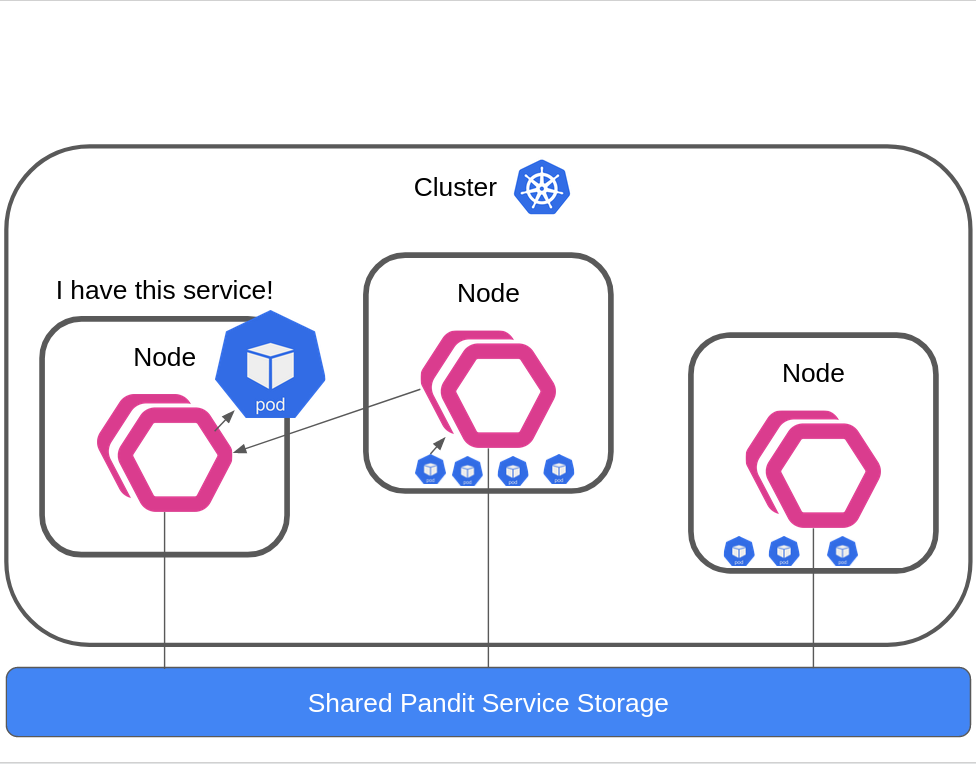
\includegraphics[width=\linewidth]{k8s.png}
    \caption{A diagram of Pandit deployed in Kubernetes. A service consisting of one Pod is announced on by the leftmost daemon. A client on the centre node subsequently sends a request to this service.}
\end{figure}
\newpage

\subsubsection{Handling Pod Termination}
Regardless of the method of deployment, Pods can be created and destroyed automatically by the Kubernetes Scheduler.
This causes a problem for Pandit because Pods may be deployed on different Nodes. In order for Pandit to be able to handle requests for data on these Pods,
it must do the following:

\begin{enumerate}
    \item Run an event loop that listens for a Pod termination event via the Kubernetes API.
    \item When a Pod is terminated, broadcast via Redis that the Pod in question has been terminated.
    \item All daemons on all Nodes will start listening for a new Pod that matches the description provided in the Service Specification. All daemons will have access to this specification because they all share a storage volume.
    \item When a daemon finds the newly created Pod, run the \textit{Add Service} command locally and announce the Pandit Service.
\end{enumerate}

This deployment mode allows for a lot of flexibility in how deployments should happen. It acts as an extension to Kubernetes itself in a way, due to tightly integrating into the Kubernetes ecosystem.

\chapter{Implementation}

In the previous chapter, the architecture of the daemon and CLI were outlined. In this chapter, the details on how this was implemented will be outlined.
\section{Fields \& Values}
\label{sec:fv}

This is the implementation of the \textbf{abstract fields representation}.

\subsection{Fields}

The implementation of \textit{Fields} is quite simple:

\begin{lstlisting}[language=Rust]
pub type FieldsMap = DashMap<String, Option<Value>>;

#[derive(Debug, Clone)]
pub struct Fields {
    pub map: FieldsMap,
}
\end{lstlisting}

It is an encapsulated map string keys to options \cite{option} of \textit{Values}.
The reason why it is a struct encapsulating a map is because it must implement traits that the underlying map does not implement.

For example, it implements Rust's built-in equality and hash trait:

\begin{lstlisting}[language=Rust]
impl std::hash::Hash for Fields {
    fn hash<H: std::hash::Hasher>(&self, state: &mut H) {
        // Build a binary heap of values in a map, ensuring they are sorted.
        let vals: BinaryHeap<Value> = self
            .map
            .iter()
            .filter_map(|entry| entry.value().clone())
            .collect();
        for val in vals.into_iter_sorted() {
            val.hash(state);
        }
    }
}

impl PartialEq for Fields {
    fn eq(&self, other: &Self) -> bool {
        // Equality of the maps is defined by hashing a sorted list of thier values and comparing them.
        let mut s_hash = DefaultHasher::new();
        self.hash(&mut s_hash);
        let mut o_hash = DefaultHasher::new();
        other.hash(&mut o_hash);
        s_hash.finish() == o_hash.finish()
    }
}
\end{lstlisting}

\subsection{Values}

\textit{Values} are integral to the abstract representation of fields. 
Implementing them proved challenging due to their unique requirements:

They must be converted to and from Protocol Buffers, as well as to and from any structured data format.

The approach chosen was to implement values as an enumeration of a set of general data types:

\begin{lstlisting}[language=Rust]
pub enum Value {
    String(String),
    Bytes(Vec<u8>),
    Int(Arc<dyn Integer>),
    Float(Arc<dyn Floating>),
    Bool(bool),
    Enum(ProtoEnum),
    Message(Fields),
    Array(Vec<Value>),
    None,
}
\end{lstlisting}

All of these data types represent one or more Protocol Buffer data types. The purpose of this is to create a general set of data types that the 
Protocol Buffer interpreter can pull from.

However, the Protocol Buffer interpreter will eventually need more concrete data types. This is particularly apparent with the integer and float data types.

These may need to be used as anything from an unsigned 8-bit integer or a signed 64-bit integer. 
These were all abstracted behind the \textit{Integer} and \textit{Floating} traits in order to simplify the conversion process on between a custom format such as JSON and a \textit{Value}.

The \textit{Integer} and \textit{Floating} traits are defined as follows:

\begin{lstlisting}[language=Rust]
pub trait Integer: Sync + Send + std::fmt::Debug {
    fn to_i32(&self) -> i32;
    fn to_i64(&self) -> i64;
    fn to_u32(&self) -> u32;
    fn to_u64(&self) -> u64;
}

pub trait Floating: Sync + Send + std::fmt::Debug {
    fn to_f32(&self) -> f32;
    fn to_f64(&self) -> f64;
}
\end{lstlisting}

These methods are designed to be implemented by any concrete data type. For example, the unsigned 64-bit integer is implemented as follows:

\begin{lstlisting}[language=Rust]
impl Integer for u64 {
    fn to_i32(&self) -> i32 {
        self.clone().try_into().unwrap_or(0)
    }

    fn to_i64(&self) -> i64 {
        self.clone().try_into().unwrap_or(0)
    }

    fn to_u32(&self) -> u32 {
        self.clone().try_into().unwrap_or(0)
    }

    fn to_u64(&self) -> u64 {
        self.clone()
    }
}
\end{lstlisting}

These methods are implemented to allow the Protocol Buffer interpreter to choose what concrete type it wants, regardless of the underlying type.
This is because the interpreter cannot be sure that, for example, the JSON parser decided to parse a "number" as a "u32" as opposed to an "i64".

\section{Serialising}

Many objects must be serialised, for example, to be transferred from one daemon to another.
The Serde library \cite{serde}.

This provides interfaces such as \textit{Serialize} and \textit{Deserialize}. They can be derived \cite{derive} for structs like so:

\begin{lstlisting}[language=Rust]
#[derive(Serialize, Deserialize)]
pub struct SQLValue(pub Vec<u8>);
\end{lstlisting}

They can also be implemented manually for a custom serialisation strategy:

\begin{lstlisting}[language=Rust]
impl Serialize for Fields {
    fn serialize<S>(
        &self,
        sr: S,
    ) -> Result<<S as serde::Serializer>::Ok, <S as serde::Serializer>::Error>
    where
        S: serde::Serializer,
    {
        use serde::ser::SerializeMap;
        let mut map = sr.serialize_map(Some(self.map.len()))?;
        for kv in &self.map {
            match kv.value() {
                Some(value) => {
                    map.serialize_entry(kv.key(), value).unwrap();
                }
                None => continue,
            }
        }
        map.end()
    }
}
\end{lstlisting}

The benefit to working with Serde is that there is an ecosystem of libraries that implement these traits.
That makes, for example, the \textit{Fields} struct interoperable with Serde libraries such as \textit{Serde JSON \cite{serde_json}}.

\section{Handler \& Writer Traits}

The \nameref{sec:writer} and \nameref{sec:handler} are just traits \cite{trait} (Rust's version of an interface).

This is the trait for the Handler:
\begin{lstlisting}[language=Rust]
#[async_trait]
pub trait Handler {
    fn from_payload(&self, buf: bytes::Bytes) -> ServiceResult<Fields>;
    async fn to_payload(&self, fields: &Fields) -> ServiceResult<bytes::Bytes>;
}
\end{lstlisting}

Each method returns a Result \cite{result}.
\textit{bytes::Bytes} is a bytes buffer. It can be used to read a series of bytes.

This is the trait for the Writer:

\begin{lstlisting}[language=Rust]
pub type WriterContext = HashMap<String, String>;

#[async_trait]
pub trait Writer: Sync + Send {
    async fn write_request(
        &mut self,
        context: WriterContext,
        fields: &Fields,
        handler: &Arc<dyn Handler + Send + Sync>,
    ) -> ServiceResult<bytes::Bytes>;
}
\end{lstlisting}

The \textit{Write Request} method takes in:
\begin{itemize}
    \item A context - This is a hash map of strings that can be used to provide extra context to specific writers. 
    For example, the hostname a HTTP header should be set to. This will all be implementation specific.
    
    \item Fields - This is the Abstract fields representation of the gRPC request.
    
    \item The \nameref{sec:handler}.
\end{itemize}

\section{Message}

The Message struct stores information on the Protocol Buffer messages.
It is stored within the Method Struct as part of a Pandit Service.

The message stores the following data:

\begin{lstlisting}[language=Rust]
#[derive(Serialize, Deserialize)]
pub struct Message {
    pub name: String,
    pub path: String,

    #[serde(skip)]
    pub parent: Arc<DashMap<String, Message>>,

    fields: DashMap<u32, Field>,
    pub fields_by_name: DashMap<String, Field>,
    pub message: protobuf::descriptor::DescriptorProto,
}
\end{lstlisting}

The \textit{parents} field maintains an Atomic Reference Counter \cite{arc} (shared reference) to the map of all messages.
This is used to aid with parsing gRPC payloads that contain nested messages. It is skipped by Serde due to it not being necessary to be serialised. 

\subsection{gRPC Payload Parsing}

The primary functionality of the Message struct is to provide methods to both write a gRPC payload from \textit{Fields} and create \textit{Fields}
from a gRPC payload.

While there is an existing set of libraries to use with Protocol Buffers, the use case this project had meant that they couldn't be used.
That's because the existing methods for using gRPC with Protocol Buffers involve generating a parsing library with code generation.

The binary \textit{protoc \cite{protoc}} is used to translate the Proto file to the required programming language. The output is then used as
a library that provides methods to run both the gRPC server and client.

\begin{figure}[hbt!]
    \centering
    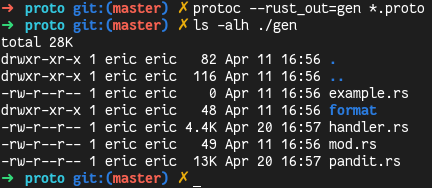
\includegraphics[width=\linewidth]{protocc.png}
    \caption{A screenshot of Protoc being used.}
    \label{fig:admin}
\end{figure}

This solution will not work for Pandit's use case, due to the Proto files being read on runtime, and running a gRPC server that is able to reflect
on multiple gRPC services on runtime.

This mean the solution was to implement the majority of the parsing logic for gRPC payload parsing from scratch, with just a few helper functions imported from existing libraries to help with interfacing with the binary directly.

Implementing the payload parsing from scratch allowed Pandit to benefit from both the flexibility provided by this solution in the form of being able to integrate it with the \textit{Fields} and \textit{Value} structs, as well as efficiency due to it all being written specifically for this use case.

\subsubsection{Challenges}

Protocol buffers consist of a series of \textbf{tags} and \textbf{binary data}.
The tag is a byte the proceeds the data. It contains a field identifier (the number defined in the Proto file) as well as the \textbf{wire type}.

A Wire Type can be best described as follows:

\begin{figure}[hbt!]
    \centering
    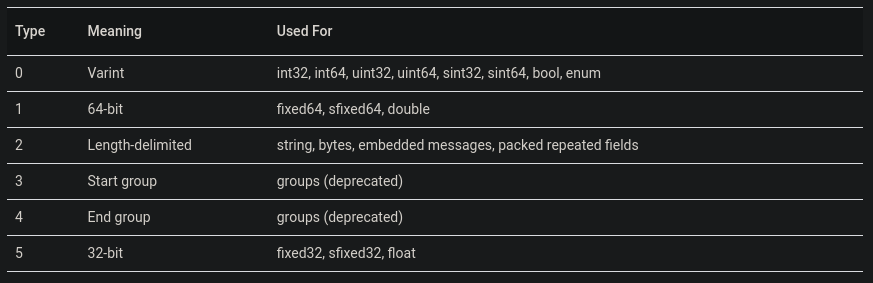
\includegraphics[width=\linewidth]{wire.png}
    \caption{A table of the different types of wire types. Copyright Google 2022. URL: \href{https://developers.google.com/protocol-buffers/docs/encoding}{https://developers.google.com/protocol-buffers/docs/encoding}}
    \label{fig:admin}
\end{figure}
\newpage

The \textit{length-delimited} wire type implies that the next byte will be the length of the coming data. This is used for all variable-length data,
including embedded messages.

The main challenges involved with implementing the gRPC payload parsers involved recursion.

When parsing embedded messages, a recursive strategy must be used. This is due to the fact that the specification requires the parser to theoretically parse embedded messages recursively ad infinitum.

The solution was to put the logic for both the reader and writer methods into a private "delimited" version of the methods.
The public methods would then call the private method, passing in the number of bytes that the parser should read to, which in the case of
the public method should be the entirety of the buffer.

\begin{lstlisting}[language=Rust]
pub fn fields_from_bytes(&self, buf: &[u8]) -> ServiceResult<Fields> {
    use std::convert::TryInto;
    let mut input = CodedInputStream::from_bytes(buf);
    input.read_raw_bytes(5)?; // Pop gRPC header.
    self.fields_from_bytes_delimited(&mut input, buf.len().try_into()?)
}
\end{lstlisting}

When the parser hits an embedded message, it will read in the length of the message, and then call a method that takes in the Proto for the field that contains the embedded, the byte stream, and the length.
It uses the aforementioned \textit{parents} field to find the specification for the method based on information provided by the field proto.
It then handles for the case of multiple embedded messages being repeated in the same field, before calling the delimited parsing method with the relevant parameters, except this time it's being called on the embedded message.

\begin{lstlisting}[language=Rust]
fn parse_another_message(
    &self,
    input: &mut CodedInputStream,
    message_name: &String,
    field: &FieldDescriptorProto,
) -> ServiceResult<Vec<Fields>> {
    use protobuf::descriptor::field_descriptor_proto::Label::*;
    let parent = self.parent.clone();
    let message = parent.get(message_name).ok_or(ServiceError::new(
        format!("no message called: {}", message_name).as_str(),
    ))?;
    let repeated_len = if field.get_label() == LABEL_REPEATED {
        input.pos() + input.read_raw_varint64()?
    } else {
        input.pos() + 1
    };
    let mut output: Vec<Fields> = Vec::with_capacity(2);
    while input.pos() < repeated_len && !input.eof()? {
        let len = input.pos() + input.read_raw_varint64()?;
        output.push(message.fields_from_bytes_delimited(input, len)?);
    }
    Ok(output)
}
\end{lstlisting}

When implementing the Protocol Buffer writer method, the \textit{\nameref{sec:fv}} proved to make the solution of handling different data types quite simple.

For example, if a method needed a 32-bit integer, this value could be received by simply calling the \textit{to-i32} method on the \textit{Integer} trait.

\begin{lstlisting}[language=Rust]
// sint32 required output.
Value::Int(v) => write_value(
    field,
    output,
    protobuf::CodedOutputStream::write_sint32_no_tag,
    v.to_i32(),
    protobuf::wire_format::WireTypeVarint,
)?,
// uint32 required output.
Value::Int(v) => write_value(
    field,
    output,
    protobuf::CodedOutputStream::write_uint32_no_tag,
    v.to_u32(),
    protobuf::wire_format::WireTypeVarint,
)?,
\end{lstlisting}

\section{HTTP/JSON Writer}
\label{im:http}

Since Pandit depends on implementations existing in the codebase of both the \nameref{sec:writer} and \nameref{sec:handler}, some example implementations were made.

One of these is HTTP/JSON also known as a REST API.

\subsection{HTTP Writer}

The HTTP Writer is an implementation of the \nameref{sec:writer} trait.
It implements the \textit{Write Request} method by:
\begin{itemize}
    \item Converting the fields to the desired payload with the \nameref{sec:handler}.
    \item Using the context provided to the method to intuit the following:
    \begin{itemize}
        \item The HTTP version of the server.
        \item The HTTP method of the request (GET, POST, etc).
        \item The full HTTP URI of the request.
    \end{itemize}
    \item Encapsulate the payload from the handler inside the HTTP headers constructed from the context.
    \item Send the request to the desired address and return the resulting payload.
\end{itemize}

\subsection{JSON Handler}
This is an implementation of the \nameref{sec:handler} trait.
It implements the \textbf{Payload to Fields} method as follows:
\begin{enumerate}
    \item Using \textit{Serde JSON \cite{serde_json}}, parse the bytes buffer of the payload into Serde JSON's \textit{Value} object.
    \item Traverse the Value tree based on the path provided to it. This will find the relevant object that will be returned.
    \item When the wanted Value is found, use Serde JSON to convert it to Pandit's \textit{Fields} struct and return.
\end{enumerate}

It implements the \textbf{Fields to Payload} as follows:
\begin{enumerate}
    \item Convert the fields to a vector of bytes by using Serde JSON.
    \item Load the vector's contents to a byte buffer and return.
\end{enumerate}

\section{Postgres Writer}
\label{im:postgres}
This is implemented in the form of both a Handler and Writer. 
For the use case of interfacing with Postgres, the Handler's purpose is converting SQL queries and responses to and from "Fields", while the Writer is used to send said queries.

\subsection{Writer}
The implementation of "Write Request" for this writer uses an asynchronous Postgres library to connect to a Postgres instance on the address provided during creation of the writer (this happens during the creation of the service).

The when a request is sent, the fields will be converted to a set of SQL commands via the Handler.

It will then send the commands to the Postgres instance. The response will come in the form of a series of "Row" structs defined in the Postgres library.

These will be serialised to a bytes buffer and returned. This is because it is the responsibility of the Handler to parse the payload.

\subsection{Handler}
The SQL handler's architecture had to be designed to work with the writer while still remaining separate components due to the architectural requirements.
The "From Payload" method converts to "Fields" by parsing the serialised payload that came from Postgres.
It goes through each row and maps its columns to the fields defined in the Pandit "Message".

It handles subsequent rows by mapping them to fields that require embedded messages. This allows Pandit to have embedded messages in SQL. 
This is achieved by building out a table of "wanted table references" and matching subsequent responses serialised in the payload by the name of their table.

The result is a fully built out "Fields". This is then returned.

The "To Payload" converts "Fields" to SQL commands. It utilises a query building library called \textit{Sea QL \cite{sea}}. 
The commands are defined in the Proto options for each method. Based on the command type chosen, different things will be added to the query builder.

Some commands such as "SELECT" require conditions. These are defined on the Proto Message fields and take the format of adding a condition enum to the field.

\section{Administration API}

\subsection{Building}

The implementation of this gRPC server first involved generating the code from the previously defined \textit{api.proto} file.
The gRPC library used for this API required a different version of the Protobuf compiler compared to the example files used to test the daemon.

Since multiple different code-gen versions were installed on the system, a Rust build script \cite{build} approach was decided on as opposed to a simple shell script. 
This allowed rust to manage the dependencies and so multiple Protobuf compilers could be installed. 

Here is the build script used:
\begin{lstlisting}[language=Rust]
fn main() {
    let proto_root = ".";
    println!("cargo:rerun-if-changed={}", proto_root);
    protoc_grpcio::compile_grpc_protos(&["api.proto"], &[proto_root], &proto_root, None)
        .expect("Failed to compile gRPC definitions!");
}
\end{lstlisting}
This will run when the rust project is being build and, if the Proto files are changed, will regenerate the code.

\subsection{Adding a Service}
The method that the API exposes allows the user to add a service to the daemon. The main process involves:

\begin{enumerate}
    \item Figure out the \nameref{sec:deployment_modes}. This will result in a mode-specific method call that will ultimately return the IP addresses of the service. If it's in Basic deployment mode, the IP address will just be the local host.
    
    \item Create the file structure that Pandit's Service constructor requires in the temporary directory. Since the Service uses a library that parses Proto files from a directory, this must be set up before the constructor is called.
    
    All of Pandit's proto library files that provide the options are embedded in the binary. They are then written to the correct file location via a static method call:
    
    \begin{lstlisting}[language=Rust]
    fn proto_libraries() -> [(&'static str, &'static [u8]); 4] {
        [
            ("pandit", include_bytes!("../proto/pandit.proto")),
            ("handler", include_bytes!("../proto/handler.proto")),
            (
                "format/http.proto",
                include_bytes!("../proto/format/http.proto"),
            ),
            (
                "format/postgres.proto",
                include_bytes!("../proto/format/postgres.proto"),
            ),
        ]
    }
    \end{lstlisting}
    
    The Proto sent via the StartServiceRequest will then be written to the directory.
    
    \item Construct the \nameref{sec:writer} based on the provided Proto file.
    
    \item Create the Service.
    
    \item Add the service to both the \nameref{sec:broker} and \nameref{sec:server}.
\end{enumerate}

\subsection{Handling Deployment Mode}
\subsubsection{Docker}

Interfacing with the Docker API is done via the library \textit{Bollard \cite{bollard}}. 
Since the deployment mode method is run from the gRPC Add Service handler, it is run from via the gRPC library's custom asynchronous context.

Rust provides asynchronous features, however, the underlying runtime that provides asynchronicity is decided by the user. This problem is that
Bollard is programmed to be used with a specific asynchronous runtime, but it has to be called from the gRPC asynchronous runtime.

The solution was to use a concept called a \textit{channel \cite{channel}}. This allows data to be transferred between threads, and hence, asynchronous runtimes.

This solution, however, required that a dedicated asynchronous listener thread to be started on startup. It would listen for requests via a channel, and return the resulting address or error via other channels.

When a request for a docker container was sent, the commands for the Docker Deployment Mode would be executed and the results returned, before being sent back via channels to the gRPC runtime.

The code that listened for requests via channels is as follows:

\begin{lstlisting}[language=Rust]
async fn run(&self) {
    loop {
        let container_id = match self.rx.recv() {
            Ok(v) => v,
            Err(err) => {
                log::error!(
                    "an error occurred receiving container id in docker network runtime: {}",
                    err
                );
                continue;
            }
        };
        match self._create_network(container_id).await {
            Ok(host) => {
                self.hosttx.send(host).unwrap(); // Send the IP address back if successful
            }
            Err(err) => {
                self.etx.send(err.to_string()).unwrap(); // Send the error if unsuccessful.
            }
        }
    }
}
\end{lstlisting}

\subsubsection{Kubernetes}
For the same reason as Docker, the Kubernetes handler also needs to be run in a separate asynchronous runtime on startup.
The main challenge when implementing this deployment mode was the fact that it had to work in a distributed environment.

The handler must figure what node(s) the service should run on (depending on the resource).
No matter what the resource being targeted is, it will always result in the querying of Pods.
These Pods will be assigned to a specific Node.

Pandit queries these nodes and constructs a set of IP addresses of the Nodes the Pods are running on.

The solution to getting the service running on each daemon, is to simply interface with each Node's Pandit daemon as a client.
The Node IP addresses will be sent a copy of the \textit{StartServiceRequest} to their own administration APIs, where they will add the Service using the same method.

The one change to the request is that the "delegated" field is set to true, telling the other nodes not to forward on the request further.

\section{Service Server}

The Service Server is responsible for handling all requests sent to Pandit services on that daemon.
The first challenge associated with implementing the server was the fact that it had to parse any gRPC request.

Usually, a gRPC server would be implemented by code generation, however, due to the aforementioned requirement, the gRPC server had to be implemented from scratch.
Since gRPC is based on HTTP/2, the server is implemented as a HTTP/2 server. After researching the abstractions gRPC introduces on top of HTTP/2,
a gRPC parser was implemented.

gRPC uses HTTP headers to define the metadata required to parse a request \cite{grpc_protocol}.
The gRPC method and service name exist in the "path" of the "URI" \cite{uris} HTTP header in the form of \textit{<package name>.<service name>/<method name>}.
These are parsed like so:

\begin{lstlisting}[language=Rust]
let path = request.uri().to_string();
let mut path = path.rsplit("/");
let method = path.next().unwrap();
let service = {
    let fqdn = path.next().unwrap();
    fqdn.rsplit(".").next().unwrap()
};
let service_name = service.to_string();
let method_name = method.to_string();
\end{lstlisting}

Another problem was how to deal with cache hits, as well as sending the query to the proxied application when needed.
The solution was to introduce a trait called a "Sender".
The \textit{Sender} trait provides a way to both send a request to a method and get a response, as well as probe cache for said method.

Here is the trait:

\begin{lstlisting}[language=Rust]
#[async_trait]
pub trait Sender: Send + Sync {
    async fn send(
        &mut self,
        service_name: &String,
        method: &String,
        data: &[u8],
    ) -> ServiceResult<bytes::Bytes>;

    async fn probe_cache(
        &self,
        service_name: &String,
        method: &String,
        data: &[u8],
    ) -> ServiceResult<Option<bytes::Bytes>>;
}
\end{lstlisting}

The underlying object is provided by the Broker. This allows the Server to exclusively interface with these methods.
If a cache probe is successful, the data will be returned to the client, or else the "Send" method will be called, and the response will be returned to the client.

\section{Services}

The Service was implemented to be a \textit{Sender}.

\subsection{Constructing a Service}

The service is constructed by parsing a Proto file using the Rust Protobuf Parse package \cite{parse}, a package generally used by the Proto to Rust compiler to generate a detailed "description" of the Proto file before compilation.

The Service was engineered to handle these "descriptors" by converting them into Pandit-specific structures, such as creating a series of method structs that pointed to an input message and output message.

The service constructs a \nameref{sec:handler} for each method based on the options set by the user. This has to be reflected on using a method that dynamically returns a Handler due to the Method struct being Handler-agnostic.

This method demonstrates how the handlers options can be parsed:

\begin{lstlisting}[language=Rust]
fn handler(
    handler: proto::gen::handler::Handler,
    path: String,
) -> Option<Arc<dyn Handler + Sync + Send + 'static>> {
    use proto::gen::handler::Handler::*;
    match handler {
        JSON => Some(Arc::new(JsonHandler::new(path))),
        _ => None,
    }
}
\end{lstlisting}

The issue was how to provide format-specific context to the handlers when implementing the "Send" method. The solution was to write a method that reflects on information available in the Service, such as options set for a specific format, and construct a "Writer Context" based on this information.

For example, here is the implementation for the HTTP format:

\begin{lstlisting}[language=Rust]
fn context_from_api(api: &Option<format::HTTP>) -> ServiceResult<WriterContext> {
    let context = WriterContext::new();
    use crate::proto::gen::format::http::http::Pattern;
    match api {
        Some(http) => match http
            .pattern
            .as_ref()
            .ok_or(ServiceError::new("no pattern in api"))?
        {
            Pattern::get(s) => {
                context.insert("method".to_string(), "GET".to_string());
                context.insert("uri".to_string(), s.clone());
            }
            Pattern::put(s) => {
                context.insert("method".to_string(), "PUT".to_string());
                context.insert("uri".to_string(), s.clone());
            }
            Pattern::post(s) => {
                context.insert("method".to_string(), "POST".to_string());
                context.insert("uri".to_string(), s.clone());
            }
            Pattern::delete(s) => {
                context.insert("method".to_string(), "DELETE".to_string());
                context.insert("uri".to_string(), s.clone());
            }
            Pattern::patch(s) => {
                context.insert("method".to_string(), "PATCH".to_string());
                context.insert("uri".to_string(), s.clone());
            }
        },
        None => {}
    }

    Ok(context)
}
\end{lstlisting}

\subsection{Handling Services on Startup}

Services must be run on startup to maintain the posterity of a service through interruptions such as restarts or redeployments.

This is achieved firstly be the \nameref{sec:api} serialising the request used to create the service to a file.

When the program starts, it then checks reads all the service files and does the following:

\begin{enumerate}
    \item Deserialise the contents of the file to a "StartServiceRequest".
    \item Ensure that the "delegated" field is set to true to ensure the request does not trigger a delegation.
    \item Send the request to the local \nameref{sec:api} endpoint.
\end{enumerate}

\section{Broker}
\subsection{Announcing a Service}
While announcing a Service does mainly entail pointing a key to the host of the daemon it's running on, it also requires the publishing of other information such as:

\begin{itemize}
    \item The default cache config for the service. This is used as a fallback cache configuration during a cache probe.
    \item A serialised map of all methods. This is used to ensue each daemon is aware of all the methods available to it.
    \item A serialised map of all messages. This was added to publish the caching strategies, as they are stored for the message in these objects.
\end{itemize}

\subsection{Publishing Cache}
When a new cache is published, the fields are serialised and sent to Redis.
The problem is that other metadata is required to enable features such as cache expiry.
The solution to this was to add a timestamp to the published data, allowing the daemons to know when a cache should expire.

There is also an edge case where some \textbf{fields} may have been disabled from being cached. 
The solution to this problem was to filter these fields out using a recursive cloning approach:

The fields would be iterated through and cloned, unless the "disabled" option was set to true. These fields would be ignored.
The challenge with this approach however was that it had to handle embedded messages recursively. This was achieved by finding the message descriptor for this embedded message (the descriptor is what stores the user-defined options) and recursively calling the "filter fields" function from there.

Here is a code snippet of the values either being cloned or recursively cloned, depending on the type:

\begin{lstlisting}[language=Rust]
match value {
    Value::Message(fields) => {
        let message_type = field_proto.descriptor.get_type_name().to_string();
        let cached = cached.parent.get(&message_type).ok_or(ServiceError::new(
            format!("no message found for type: {}", entry.key()).as_str(),
        ))?;
        map.insert(
            entry.key().clone(),
            Some(Value::Message(self.filter_fields(fields, cached.value())?)),
        );
    }
    v => {
        map.insert(entry.key().clone(), Some(v.clone()));
    }
};
\end{lstlisting}

\subsection{Receiving Cache}
The Broker is implemented to run from startup. It will connect to a Redis instance and start listening for updates to the PUB/SUB database using an event loop.

When a value is received, it will decide what type of update it is based on the name. For example, when the cache is published and the daemon is subscribed, the solution to parsing this cache is to deserialize the payload. The deserialized values include the timestamp that the cache was created at. 

Along with the cache expiry time, this can be used to check if a cache is expired. Here is a sample of the code that handles this:

\begin{lstlisting}[language=Rust]
let (primary_key, payload): (Value, Vec<u8>) =
    serde_json::from_slice(msg.get_payload_bytes())?;
let fields_map = cached.fields_for_key.clone();
let cached_fields = CachedFields {
    data: bytes::Bytes::copy_from_slice(&payload[..]),
    fields: cached.message.fields_from_bytes(&payload[..])?,
    timestamp: SystemTime::now(),
};
fields_map.insert(primary_key.clone(), cached_fields);
cached.fields_for_key = fields_map;
self.method_fields_map.insert(name.clone(), cached);
log::info!(
    "cache updated for {}: primary key value = {:?}",
    &name,
    &primary_key
);
\end{lstlisting}

\subsection{Probing Cache}

Cache probing is triggered by the \nameref{sec:server} by calling the \textit{Probe Cache} method on a \textit{Sender}.
A \textit{Service} implements this method by parsing the method and service names, then finding the primary key and delegating the request to the Broker.

The Broker does a simple cache lookup, ensuring the cache exists and is in date, or else returns "None".

However, when a Service is not on the local daemon, there is no service object to use. In this case, the Service Server queries the broker for cache for a specific Service. The broker will construct return a "Remote Sender". An implementation of the Sender that fulfils the following purposes:

\begin{itemize}
    \item When queried for cache, it will look interface with the broker's cache table to find the latest cache, ensuring it is in date.
    \item If the server doesn't find cache and wants to send the query to the proxied application via the "send" method, the remote sender will instead send the raw query to the daemon that hosts the Service, delegating the query.
\end{itemize}

\section{CLI}
The Command Line Interface is implemented using a CLI library called \textit{clap \cite{clap}}.

The main challenge experienced when implementing the CLI involved the package installation process.
Since the packages were defined in a remote JSON file, a series of structs were made to represent them. These were used to deserialise the JSON stream.

\begin{lstlisting}[language=Rust]
#[derive(Deserialize, Serialize)]
pub struct Index {
    pub packages: HashMap<String, Package>,
}

#[derive(Deserialize, Serialize)]
pub struct Package {
    pub version: String,
    pub proto_url: String,
    pub image: Option<Image>,
    pub readme_url: Option<String>,
    pub logo_url: Option<String>,
}

#[derive(Deserialize, Serialize)]
#[serde(tag = "type")]
pub enum Image {
    Helm {
        repo_url: String,
        repo_name: String,
        chart: String,
        container_name: Option<String>,
    },
    Docker {
        compose_file: String,
    },
}
\end{lstlisting}

When installing a package, the optional "image" provided a way to install a resource in either Docker or Kubernetes.

If the Docker config was present, it would link to a Docker Compose \cite{compose} file. This is a YAML file that provides a method of deployment for Docker containers. The solution here was to create a docker compose file in the local filesystem alongside the Proto file. Docker Compose would then be called to deploy the Docker containers.

Helm \cite{helm} is a package manager for Kubernetes resources. It provides deployment files from a remote location.
When this option is chosen in the package, the CLI will interface with the local helm instance to both download and install the relevant package.
Integrating this into the CLI was challenging, since a progress bar was implemented to show the user the progress of the installation.
This required the integration of a package called \textit{Indicatif \cite{indicatif}} to the CLI.

\chapter{Evaluation}
\section{Unit Testing}
Many unit tests were implemented to test the functionality of the components of the daemon.

\subsection{Messages}
The \textit{\nameref{sec:messages}} methods used to parse Protobuf payloads were tested to ensure that they provided the correct
data to the rest of the program. This was done because there was no feasible way of reliably testing this functionality manually.

The Protobuf writer test was implemented as a "table" of tests. This is a design pattern that involves creating a structure that represents a set of test parameters and filling out those fields with different values that increase coverage of the tests.
The structure used was as follows:

\begin{lstlisting}[language=Rust]
struct Table {
    name: String,
    field_type: Type,
    number: i32,
    type_name: String,
    label: Label,
    value: Value,
}
\end{lstlisting}

Since the action of writing a field to the bytes buffer is atomic, the field values in each table are put into a single "Fields" object and sent to the method.
The buffer is then checked against the desired value after the test is executed to ensure it behaved properly

The reading of a Protobuf to the "Fields" object was tested by constructing a desired "Fields" object alongside a hardcoded Protobuf payload:
\begin{lstlisting}[language=Rust]
let buf: &[u8] = &[
    0, 0, 0, 0, 0, // gRPC header.
    0x08, 0x96, 0x01, // Field varint
    0x12, 0x07, 0x74, 0x65, 0x73, 0x74, 0x69, 0x6e, 0x67, // Field string
    0x1a, 0x03, 0x08, 0x96, 0x01, // Embedded message
    0x22, 0x08, 0x03, 0x08, 0x96, 0x01, 0x03, 0x08, 0x96,
    0x01, // Embedded message repeated x2
];
\end{lstlisting}

The "Field" object is provided to the method and the output is checked against the hardcoded payload.

\subsection{Service}
The \textit{\nameref{sec:service}} was also tested to ensure that it called a \textit{\nameref{sec:writer}} when a query was made.
This was done by creating a fake \nameref{sec:writer} in order to ensure that a payload was sent to the desired application. 

A Service is created with all the necessary values passed to it, including a sample Proto file that was made for testing purposes.
The "Send" method is then called with the necessary parameters. 

Finally, the values sent to the fake Writer are checked to ensure the method works correctly.

\section{System Testing}
\label{sec:test}
\subsection{Basic Deployment}
In order to ensure the daemon was working correctly, a fake REST API was implemented in python to serve as an authoritative container.
A Protobuf specification was created for the API, and it was passed to the daemon via \textit{\nameref{sec:cli}}.

The Protobuf specification was used to generate a Rust client library \cite{codegen} that was used to interact with the daemon.
A standalone testing binary was implemented by importing this library and calling the service in question.
It sent the same query twice, the first time it was ensured that the data came directly from the authoritative container, and the second time it was
ensured that the data came from the cache.

\subsection{Docker Deployment}
The sample application as well as the Pandit daemon were put inside Docker images and deployed to docker containers. 
They were deployed using a Docker Compose \cite{compose} file:
\begin{lstlisting}
version: '3.9'
services:
  redis:
    image: redis
    networks:
      - redis

  example:
    build: src/proto/examples
    entrypoint: "python /example_rest.py"

  pandit:
    build: .
    depends_on:
      - redis
    ports:
      - "50122:50122"
      - "50121:50121"
    entrypoint: "/panditd --docker"
    volumes:
      - /var/run/docker.sock:/var/run/docker.sock
    networks:
      - redis

networks:
  redis:
\end{lstlisting}

The docker socket was passed to the Pandit container to allow it to query and modify the Docker state.
Then, the example service used in the basic deployment was deployed and tested.

\subsection{Kubernetes}
A Kubernetes cluster was deployed locally using a tool called \textit{Minikube \cite{kube}}. 
The resources were deployed using a series of deployment scripts, which take the form of YAML files.
The Minikube cluster deployed 3 virtual machines as 3 nodes in the cluster.

These files deployed a Pandit daemon on each host in the form of a "DaemonSet".
They also deployed a Redis Pod and Service, as well as an example application to be proxied in the form of the aforementioned REST API.
A Pod to use as an example client was also deployed.

The Pandit deployment also got access to specific API features by allowing the default user to access said endpoints:

\begin{lstlisting}
---
apiVersion: rbac.authorization.k8s.io/v1
kind: ClusterRole
metadata:
  namespace: default
  name: pod-reader
rules:
  - apiGroups: [""] 
    resources: ["pods", "nodes"]
    verbs: ["get", "watch", "list"]
---
apiVersion: rbac.authorization.k8s.io/v1
kind: ClusterRoleBinding
metadata:
  name: read-pods
  namespace: default
subjects:
  - kind: "ServiceAccount"
    name: "default"
    namespace: "default"
roleRef:
  kind: ClusterRole 
  name: pod-reader 
  apiGroup: rbac.authorization.k8s.io
\end{lstlisting}

The CLI was then used to interface with a Pandit daemon on a single host whilst the Pod was on another host. This to validate that a Service could be added to a specific node from another node.

An example client was used from a Pod on another node to test Pandit's query delegation. 

Another feature that was tested was Pod eviction handling. Upon first try, the feature was very buggy and difficult to debug. The daemons running on each node required a lot of debug information to be logged in order to understand how they listen for state changes in Pods.

After days of testing, bug fixing and recompiling, the feature began to work as expected, allowing services to move between Nodes as the Pods's states change.

\subsection{Handlers and Writers}

Due to time constraints, most of the testing was focused on the deployment modes using a HTTP/JSON application.
Testing also takes a long time due to the requirement of building a sample application and client.
For this reason, the SQL writer and handler are not confirmed to be fully functional, however, some functionality was tested, such as 
SELECT statements on a Postgres database. A sample Proto file was also made to ensure the Service can successfully construct an SQL Handler:

\begin{lstlisting}
message ExampleTable {
  int32 id = 1 [ (pandit.key) = true, (pandit.format.postgres_field) = {key : true} ];
  string name = 2;
}

message Empty {
}

service PostgreSQL {
  option (pandit.name) = "postgres";
  option (pandit.format.postgres_service) = {
  };

  rpc SetExample(ExampleTable) returns (Empty) {
    option (pandit.format.postgres) = {
      command : INSERT
    };
    option (pandit.cache) = {
      cache_time : 3000
    };
  }

  rpc GetExample(ExampleTable) returns (ExampleTable) {
    option (pandit.format.postgres) = {
      command : SELECT
    };
    option (pandit.cache) = {
      cache_time : 4000
    };
  }
}
\end{lstlisting}

\section{Appraisal}
This project went through many iterations, both in concept and implementation.

It was originally conceptualised as a proxy that performed kernel-level packet parsing (using eBPF \cite{ebpf}), ultimately providing a distributed gRPC service.
After working on a sample implementation of the eBPF code, the problems associated with eBPF in the \textit{\nameref{sec:ebpf}} section became apparent.

After deciding on doing all packet parsing in user space, the project began to take form.
C++ was originally the language being used to implement the user space code, however, the implementation was switched to Rust due to it having a more suitable set of libraries available to it when it came to implementing the gRPC server.

\subsection{Does Pandit meet the Objectives?}

Despite deviations in approaches, the \nameref{sec:objectives} always stayed the same.
This is where the final implementation stands in relation to these objectives:

\begin{itemize}
    \item The final product's architecture enables developers to easily integrate new data formats into Pandit. 
    All a developer needs to do is provide implementations for the traits \nameref{sec:writer} and \nameref{sec:handler}.
    
    These traits should allow developers to implement support for any data format they require, as demonstrated by the existing implementations of the \nameref{im:http} and \nameref{im:postgres}. 
    JSON being a text-based object notation and Postgres being a Structured Query Language mean that these two implementations differ wildly in how they interface with applications.
    But since the fact that they are both interfaced with by the rest of the Pandit components behind the same trait shows that the architecture meets the objective: being able to proxy any data source.
    
    \item Another objective was the ability to provide a Pandit \nameref{sec:service}. This objective was met when the \nameref{sec:service} and \nameref{sec:server} components were implemented. 
    However, outside unit tests, the product was only able to verified to work after the \nameref{sec:api} was implemented as this is what allows users to add services.
    
    \item Pandit achieves the objective "Using Protobuf Options, Pandit should provide a way to define the conversion between the application and the Pandit Service" for the most part.
    
    Users can define how conversions are done by importing the provided Proto files. 
    They are able to get around edge cases such as the required object being a child of the object returned by the application via a "path" option available on each message.
    
    Overall this provides a decent user experience, however, the limitations of \nameref{sec:options} are apparent in some ways when writing a service. 
    For example, the amount of copied and pasted syntax and repetition required to implement a message is more than desirable.
    This is particularly evident with the primary key, which requires the following option to be attached to a field in every request message:
    \begin{lstlisting}
    message ExampleRequest {
      // Primary key:
      int32 id = 1 [ (pandit.key) = true ];
      string user = 2;
    }
    \end{lstlisting}
    
    \item The objective to allow for user-defined caching strategies was met by providing options for users to configure how entire messages as well as individual fields can be cached.
    However, in terms of feature-set, it is quite limited due to the fact that the caching features are primarily a proof of concept.
    
    Currently, the only available caching options are the following:
    \begin{lstlisting}
    message CacheOptions {
      bool disable = 60031; // If set, disables the target from being cached.
      uint64 cache_time = 60032; // If set, the cache will expire after this amount of seconds.
    }
    \end{lstlisting}
    This was deemed sufficient due to the scope of this project, however, given more time many more options would be added.
    These could include a way to define more complex associations between fields. 
    Right not the only way to get a cache hit is with a matching primary key. 
    A more flexible (and technically challenging) approach would be to allow users to define cache hits via conditions such as:
    \begin{lstlisting}
    if field_a > field_b:
        cache hit
    else if field_c exists:
        cache hit
    \end{lstlisting}
    
    \item Pandit is able to run in a cluster of servers whilst coordinating requests between servers due to every server being connected to a message broker.
    It is confirmed to be working sufficiently during the aforementioned system \nameref{sec:test}. 
    
    The deployment of Pandit in a distributed environment requires prerequisite knowledge of the cluster's network architecture, and so isn't designed to be easy to installed out of the box. 
    It is instead designed to be deployed by an engineer familiar with the cluster, and to that end, it has met this objective.
    
\end{itemize}

\subsection{Qualitative Evaluation}
\label{sec:qual}
\subsubsection{Caching}
Compared to other industry solutions such as those mentioned in \nameref{sec:solutions}, Pandit in its current form provides a set of features that stand out from the competition.

The caching features have limitations, however. Pandit assumes that when an object is cached, the underlying data will not change, i.e. the underlying methods are deterministic. This is because maintaining coherency between the cache and the underlying data is a problem outside the scope of this project.

Since the user is responsible for defining how and what should be proxied, Pandit has no way of knowing what is happening on the application outside the snippets of information it gets from the query responses. 
This means, if information changes due to an action handled outside of Pandit, there is no way to maintain consistency between the application and daemon.

\textit{See \nameref{sec:future} for possible solutions to this problem.}

\subsubsection{Feature Set}
The feature set of Pandit in its current form can best be described as a proof of concept.
However, its architecture allows it to be both easily extended and deployed in many environments.
Therefore, it could be integrated into a production environment if a company wanted to benefit from its current feature set.

The ability to turn any application into a gRPC service without any modification of the application's source code is something many companies would see value in.
This is due to the innate benefits of a gRPC service over other data formats, such as:
being able to generate a client library in any language \cite{codegen}. 

Pandit integrates basic package management functionality into its \nameref{sec:cli}. 
This feature could be used to interface with an internal repository of Proto files inside a company.
When a developer needs to implement a client for a particular service, they could simply use Pandit to both download the relevant Proto file 
and deploy a local version of the application for testing.
A system administrator can use the same feature to install the relevant Proto files in a production environment. 
They can subsequently use said Proto files to deploy services to Pandit.
Therefore, this feature allows there to be an ecosystem of Pandit packages that simplify both development time and deployment.

As outlined in \nameref{sec:deployment_modes}, Pandit integrates into industry standard deployment models such as Docker and Kubernetes. 
Since these technologies are widely adopted within the industry, most companies could integrate Pandit into their existing software stack.

\subsubsection{Comparison to Other Solutions}
\label{sec:comp}
As mentioned in the \nameref{sec:solutions} section, there are alternative solutions to Pandit.
Here we will compare Pandit in its current form to these solutions.

\begin{itemize}
    \item Pandit provides similar functionality to \textit{Google Cloud Endpoints with HTTP/JSON to gRPC encoding \cite{cloud_endpoints}}; but Pandit provides far more flexibility due to its ability to translate any data format.
    Both Pandit and Google Cloud's solution translate HTTP/JSON to gRPC. Pandit's support for HTTP/JSON is fully tested with an example application.
    This makes Pandit's current feature set subsume the features provided by Google Cloud's solution. 
    This is because Pandit also includes the ability to define custom caching strategies. 
    Pandit can also be deployed inside any distributed system, while Google Cloud's solution is exclusively available in Google Cloud.
    
    \item \textit{Envoy Proxy \cite{envoy}} has a different approach to proxying than Pandit.
    It runs an instance of itself alongside each application, inside the same container.
    It also only performs translation between application layers, such as "HTTP/1.1 to HTTP/2".
    
    Pandit is implemented to run on each node, reducing the amount of instances that must be deployed compared to Envoy.
    
    Pandit also translates the application into a gRPC service. This allows for a different approach to caching compared to Envoy.
    Envoy caches HTTP queries by exclusively parsing the HTTP headers. This means it indexes its in-memory cache exclusively by URI.
    Pandit on the other hand maintains a cache based on a user-defined field sent in via gRPC.
    This provides more flexibility in defining caching strategies as it is more configurable.
\end{itemize}

\section{Summary}
\textit{Pandit} is a great tool for caching and querying data in a distributed system.
It also provides a great deal of flexibility for users to define their own caching and querying strategies.

Whether it be a REST API or an SQL Database, all it takes is a single Protobuf specification \cite{protobuf} to turn it into a
\textbf{widely available gRPC \cite{grpc} Service}. Services become widely available due to the caching mechanism in the daemon being on every host,
as well as the publish/subscribe mechanism used to distribute the cache to all interested daemons.

The fact that anything can be turned into a gRPC service provides a lot more flexibility to the users of the product compared to any existing solution.
This is because you can build a client library for any language or framework using a Protobuf \cite{codegen}.

This also means that Pandit has innate benefits for any application that requires data from other services.
For example, instead of using an ORM \cite{orm} and manually encoding the data to be read in the application, you can use Pandit to
to turn the database into a gRPC service and then use the gRPC client library to read the data. This will give you the added benefit of
being able to cache the data and query it in a distributed system if it needs to be deployed to multiple hosts later on.
You could also implement another client in a different language in one step by generating code from the Protobuf \cite{codegen}.

Pandit also requires no configuration of the application being proxied. As long as pandit has the service added, it will be ready to accept requests.
This is because the daemon interfaces with the application as a client.

Overall, Pandit's quality is fitting of a proof of concept. 
It demonstrates the possibilities of this approach to distributing services, meeting the objectives set for it.
It is not ready to be deployed in a production environment, however, as far more testing would be required, especially in the areas of stability and performance.

Pandit in its current form could find success as an open-source project, where it would benefit from having many eyes on it, reducing the likelihood of it experiencing bugs and instability.

All in all, Pandit has the potential to be a very useful product, providing practical solutions to problems companies are currently experiencing when deploying their applications to distributed systems.

\chapter{Conclusions}

\section{Reflection}
I have learned many things throughout the research, design and implementation of this project.
I have learned the Rust Programming Language \cite{rust}: an up-and-coming programming language that has many innovative and exciting features.

I also learned the core concepts behind Kubernetes \cite{k8s} such as Pods, Deployments, Resources, etc. I also learned how to write an application
that works inside Kubernetes.

During the early days of my research, I focused primarily on how packets can be parsed in eBPF \cite{ebpf} (see \nameref{sec:ebpf} for more details).
I spent a long time trying to get a solution in code.
This proved to be a dead end due to eBPF's limitations, and the approach was scrapped. 
If I could start again, I would weigh the ups and downs of multiple approaches from the start and make a decision based on the objectives of the project.

After modifying my approach to interface with the application in user space (see \textit{\nameref{sec:user}} for more details), development went a lot smoother.

Overall, I learned a lot of skills both technical and non-technical that will really help me in the future. I have learned from my mistakes in the planning phase, which has taught me how to approach project planning in the future.

\newpage
\section{How the project was conducted}
\begin{figure}[hbt!]
    \centering
    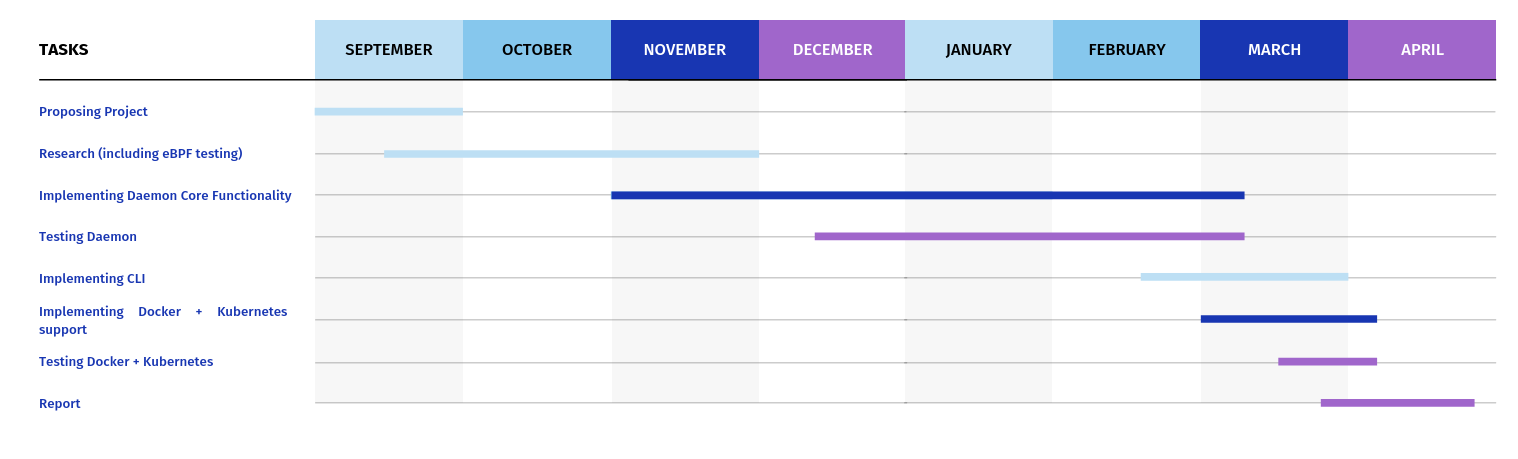
\includegraphics[width=\linewidth]{gantt.png}
    \caption{A Gantt chart showing the time taken to do each general task.}
\end{figure}

A lot of thought was put into the initial project proposal. After the project was accepted by Professor Dirk Pesch, research began.

As stated above, a lot of research went into the area of eBPF. After this approach was scrapped, research began in areas such as gRPC and The Rust Programming Language.

During the research phase, implementation of the daemon's core features began. This included implementing the \nameref{sec:service}, \nameref{sec:messages}, \nameref{sec:handler}, \nameref{sec:broker} and \nameref{sec:writer} components.

After a basic version of a component, such Service was completed, testing began alongside further development. This allowed bugs to be found whilst development continued.
This section of development was the largest bottleneck in the development process due to the complexity and scope of the task.
If the project was started again, this stage would have been started much sooner to allow for ample time to complete the rest of the tasks.

\nameref{sec:cli} began development in mid-February, alongside the \nameref{sec:api} in the daemon. After the "Install" method was completed,
the Kubernetes/Docker Deployment modes began development. Development after this switched between Kubernetes and the CLI, to ensure the product could be deployed.

During the end of development, work on the report started. After the open day, all work was focused on the report.
Due to the complexities involved in implementing this project, the report necessitated lots of length explanations, increasing the workload in April.
If this project was started again, the report would be done alongside the implementation stage, reducing the stress involved in writing the report in April.

\section{Future Work}
\label{sec:future}
\subsection{Solutions to Caching Problems}
In the \nameref{sec:qual}, the problems associated with caching were introduced.
A possible solution to some of these issues could involve a user-defined refresh time. For example, if it is known that a particular value is mutated on a recurring daily interval, such as every day at 1am, the user could configure Pandit to either invalidate the cache at 1am or query for an updated version of the cache.
This solution would likely be implemented given more time.

There are still coherency issues with this solution if there is no set interval for mutations of the data.
In its current form, the user would be advised to either disable caching on these methods. They would still benefit from the gRPC translation aspects of the project.

A solution that could solve this may involve a callback method the application can avail of that will notify Pandit of changes to the data.
This would have many issues and is in conflict with one of the core selling points of the project: "the application should not need to be modified in order to work with Pandit".
Since there was no desired solution to this problem, it was deemed outside the scope of this project.

\subsection{CLI/Ecosystem improvements}
\nameref{sec:cli} currently supports a very basic install operation. 
It simply reads from a remote JSON file, looks for the package, and downloads the necessary files.

If more time was granted, the CLI would be designed to pull from a fully implemented API. 
The API would provide server-side authentication, a way to upload/update packages, as well as many other features.

A Web UI was set as a stretch goal; it would demonstrate how a user could download packages by copying a command from a website.
An implementation was started but was set aside and later removed due to time constraints. 
If more time was granted, a full website would be made.
It would allow users to manage and upload packages, as well as discover new packages.


\medskip

\chapter*{Terminology}

\printbibliography


\end{document}